%!TEX root = thesis_cgo.tex
\chapter{Conformational analysis of the \tub carboxyl terminus}

\epigraph{Only in disorder are we conceivable.}{Roberto Bola\~no}

In this chapter we discuss the impact of phosphorylation on the global dynamics of the \tub C-terminus (\gct). We begin with the finding that the \gct has been shown to be phosphorylated {\it in vivo} ~\cite{keck2011cell}, and mimicking constitutive phosphorylation of a conserved tyrosine residue in the \gct perturbs the function of the mitotic spindle~\cite{vogel2001phosphorylation}. We therefore hypothesize  that  transient phosphorylation at  the \gct IDR  is acting  to  regulate an as of yet unknown aspect of the function of the spindle via a structural mechanism. More specifically, we will be studying  the highly conserved tyrosine 11 (Y11) of the \gct where we study the IDR which has been identified as a key phospho-site  in this system ~\cite{vogel2001phosphorylation}. This is a first step towards describing a molecular mechanism by which regulation of the \gct promotes proper spindle function and the identification of key residues involved in binding molecular partners. 

In order to understand the effect of phosphorylation at Y11, we took two approaches. First, NMR experiments provide critical structural information; including translational diffusion coeffecients, fast motions at nsec timescales that correspond to sidechain dynamics as well as slow motions of the backbone that correspond to dispersion, and the timescale of exchange between states. Collectively, these NMR experiments are used to probe the conformational sampling  of non-phosphorylated  and  phophomimetic forms of the  \gct. These experiments revealed slow motions and exchange between two states that are only observed in the Y11D mutant.  Thus molecular dynamics simulations were employed gain deeper insight regarding the observed comformational sampling. Because phosphorylation is  a challenge to  implement  controllably  \vivo and \vitro, we approximate the electrostatic  effects of a phosphorylation by introducing an acidic residue, Aspartic  Acid (D),  at  the phosphorylation site through site directed mutagenesis. We therefore study the wild-type sequence, WT: \texttt{LLRGAAEQDSYLDDVLVDDENMVGELEEDLDADGDHKLV}, and the phospho-mutant Y11D: \texttt{LLRGAAEQDSDLDDVLVDDENMVGELEEDLDADGDHKLV} using MD simulations. By comparing results from our simulations to experimental measurements previously performed with NMR spectroscopy on the \gct, we are able to propose that local changes in charge at the 11 residue in the polypeptide modulate the conformational sampling of the \gct. The changes in conformational sampling we observe point to a physical mechanism for regulating the availability of binding surfaces on \tub. Furthermore, we describe a novel mode of IDP control whereby functionality arises from switch-like transitions that lie entirely within disordered states.

\section{NMR}

NMR experiments were done by collaborators in the Department of Chemistry at McGill on the WT and YD forms of the \gct. Through protein NMR spectroscopy we are able to obtain accurate \vitro measurements of the structural and dynamic properties of polypeptides. Among these are secondary structure state, dynamic conformational changes, and structural properties such as diffusion rates. Given that the \gct is intrinsically disordered and therefore highly dynamic, this makes NMR a particularly well suited to this problem. Diffusion measurements show that the major conformation of both forms corresponds to that of a collapsed polypeptide. By computing the effective hydrodynamic radius of the polypeptides using the Stokes-Einstein ~\ref{eq:stokes} we can compare the compactness of the \gct to other known structures. The for WT we obtain \diffusion=\num{1.25e-6} $\pm$  \SI{1e-8}{\dcunits}, $r = \SI{14.2}{\angstrom} \pm 0.2$ and \diffusion= \num{1.224e-6} $\pm$ \SI{3.503e-8}{\dcunits}, $r = \SI{15.6}{\angstrom} \pm 0.2$ for the YD mutant. Both are close to the hydrodynamic radius of the folded fibronectin binding protein D3 ($r = \SI{14.9}{\angstrom}$) ~\cite{wilkins1999hydrodynamic} and well under the predicted Stokes radius of an extended 39 amino acid chain \todo{ref nmr fig}. This is a surprising finding given the high content of negatively charged residues (15 of 39 residues) in both forms would be expected to promote open conformations. However, because that the \gct also has a relatively high number of hydrophobic residues (14/39), it is likely that there are other forces, such as the hydrophobic effect, acting on the packing of the peptide. We also note that the YD has a slightly higher Stokes radius than the YD suggesting some shifts in conformational sampling that are absent in the WT. Chemical shift secondary structure predictions show that both forms occupy a disordered random coil state and do not show evidence of adopting any secondary structure domains \todo{ref appendix}. Therefore, we do not observe any disorder-order transitions which are common in functionally-coupled phosphorylated IDPs. However, relaxation-dispersion experiments, which detect changes in the chemical environment of residues on the micro-millisecond timescale, show that the Y11D mutant undergoes large coordinated transitions between two states, while the WT dispersion profile is flat. The two states explored by the mutant are calculated to exchange between a major state populated to 97.5 \% and a minor state populated to 2.5\% with an exchange rate of \SI{2252}{\sec^{-1}}. Combining the dispersions brought about by the YD mutation with the shift in global \diffusion to more open conformations, we hypothesize that the YD mutation induces collective motions between a collapsed major state and an extended minor state. 

In this work we use MD simulations of both \gct forms to gain further insight into the transition hypothesized by NMR.  

\section{MD simulation set-up}

Molecular Dynamics simulations (MDS) on WT and Y11D \gct were carried out using MPI-enabled GROMACS 4.6.6 software\cite{hess2008gromacs} and a CentOS 5 high performance computational cluster. Calculations were distributed over 64 Dual Sandy Bridge 8-core, 2.6 GHz computing nodes and run under periodic boundary conditions with the OPLS-AA (Optimized Potential for Liquid Simulations All Atom) force field ~\cite{kaminski2001evaluation}.  The starting \gct polypeptide configurations were obtained from secondary and tertiary structure predictions by RaptorX \cite{kallberg2012template} and solvated using the SPCE (extended single point charge) water model in a dodecahedral box while enforcing a minimum distance between the edge of the box and solute of 1 nanometer. The total charge of the system was neutralized by adding sodium ions to the solution. Energy minimization was carried out using a steepest descent algorithm for a maximum of 50,000 steps until a maximum force of 100 kJ/mol between atoms was achieved. A 1 nm cut-off was used for non-bonded interactions, and long-range electrostatics were calculated using a Particle Mesh Edwald Sum algorithm. The systems equilibrated under the constant NVT and NPT ensembles (288K and 1 atm) for 5 ns before the production 2 $\mu$s simulations. Post-processing of all trajectories was done using the \texttt{trjconv} module of GROMACS. Theoretical random-coil structural ensembles (10,000 conformers) were calculated based on the \gct primary amino acid sequence using Flexible Meccano software \cite{ozenne2012flexible}. Translational diffusion coefficients were calculated for each structure using hydroNMR software \cite{de2000hydronmr}. 
MD conformations were grouped into percentile classes based on radius of gyration (Rg) computed using the GROMACS \texttt{g\_gyrate} module. Each Rg percentile group was represented by the three structures with lowest root-mean-squared-difference RMSD values to all other structures, calculated using the GROMACS \texttt{g\_rms} module. Atomic distance matrices were calculated using the GROMACS \texttt{g\_mdmat} module.


\section{Conformational sampling of \gct isoforms}

We computed atomic trajectories for the WT and YD forms of the \gct in all-atom MD simulations with durations of \SI{2}{\us}. We choose this simulation length because timescale of transitions observed in NMR are on the micro-millisecond order. While our nano-microsecond MD simulations do not reach such timescales due to computational limitations, long timescale motions measured in NMR have been reproduced in shorter timescale MD simulations of faster exchange rates ~/cite{massi2004nmr, stafford2015conformational, henzler2007dynamic}. From the resulting trajectories we are able to capture dynamics and conformational sampling that are remarkably consistent with those measured in NMR.\\


{\it \gct does not adopt any stable secondary structure}

The first question we addressed was whether the structures in our MD trajectories feature the same lack of global structure that was observed in NMR. We used the \texttt{dssp} algorithm ~\cite{kabsch1983dictionary} in the VMD software package ~\cite{humphrey1996vmd} to compute secondary structure assignments on each residue in the chain. Assignments by \texttt{dssp} are based on computations of hydrogen bonding energies between all atoms. Since hydrogen bonds are the primary stabilizing interaction that gives rise to backbone secondary structure, \texttt{dssp} is able to classify geometries arising from potential hydrogen bonds to a category of secondary structure motif found in a large database of annotated structures. We apply this algorithm to every frame in the trajectories at \SI{1}{\ns} intervals to assess secondary structure motifs at every residue as a function of simulation time \figref{fig:ss}. Apart from some local helicity in the middle residues, secondary structure assignment plots for all four trajectories point to a consistent absence of global secondary structure motif. The major classes of secondary structure present are turn and coil geometries which correspond to a largely unstructured ensemble of conformations. 

\begin{figure}
	\centering     %%% not \center
	\subfigure[WT]{\label{fig:ss_a}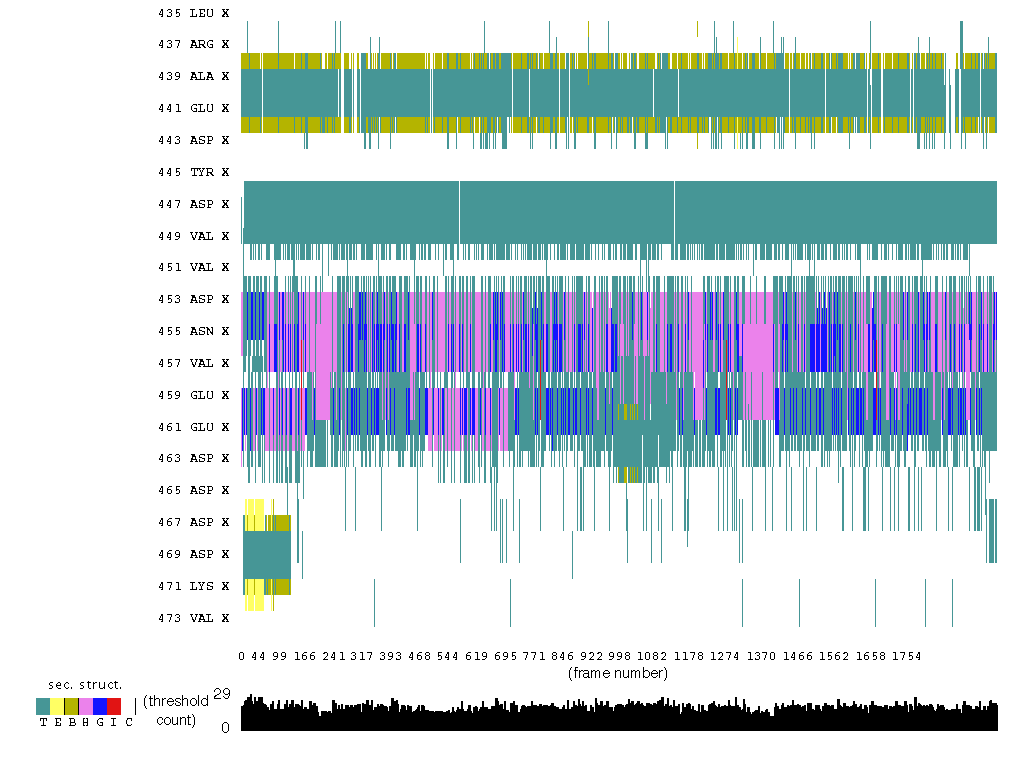
\includegraphics[width=0.49\textwidth]{wt_ss}}
	\subfigure[YD]{\label{fig:ss_b}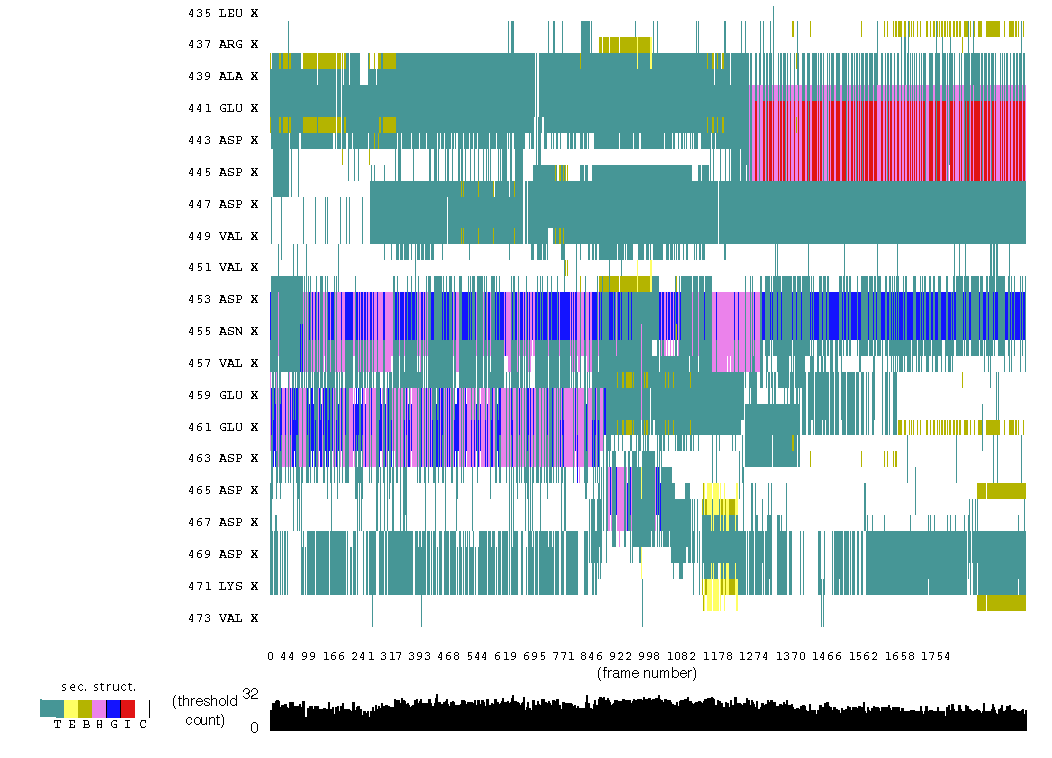
\includegraphics[width=0.49\textwidth]{yd_ss}}
	\FigureCaption{\gct Secondary Structure Assignments}{Per-residue secondary structure assignments based on 3D coordinates are computed for every frame of the simulation. WT and YD trajectories lack global and persistent secondary structure motifs throughout the duration of the simulation. Apart from turn motifs and small local $\alpha$-helices, the \gct samples largely disordered conformations and does not undergo any disorder-order transitions. T: turn, E: extended, B: isolated bridge, H: $\alpha$-helix, G: 3/10 Helix, I: $\pi$-helix, C: coil.}
	\label{fig:ss}
\end{figure}	


Although we do not observe ordered secondary structure rearrangements by looking at \texttt{dssp}, we compute RMSD to ask whether the simulations produce any conformational changes in the disordered ensemble. RMSD quantifies the distance between superimposed structures and is therefore a useful tool for detecting the presence of conformational changes in a trajectory. We therefore computed backbone RMSD values for every frame in the simulation with respect to the starting structure. Since the starting conformation is not derived from experimental data and is not expected to correspond to a native state, we also compute RMSD with a 10ns sliding window where every frame is compared with the one 10ns before. In the middle portion of the YD simulation, both methods of computing RMSD contain sharp peaks which indicate the presence of large scale backbone rearrangements \figref{fig:rmsd}. In contrast, WT RMSD values remain stable throughout the simulation. This suggests that the YD mutation can modulate conformational exploration and the stability of the \gct. 


\begin{figure}
	\centering     %%% not \center
	\subfigure[RMSD to initial frame]{\label{fig:rmsdinitial}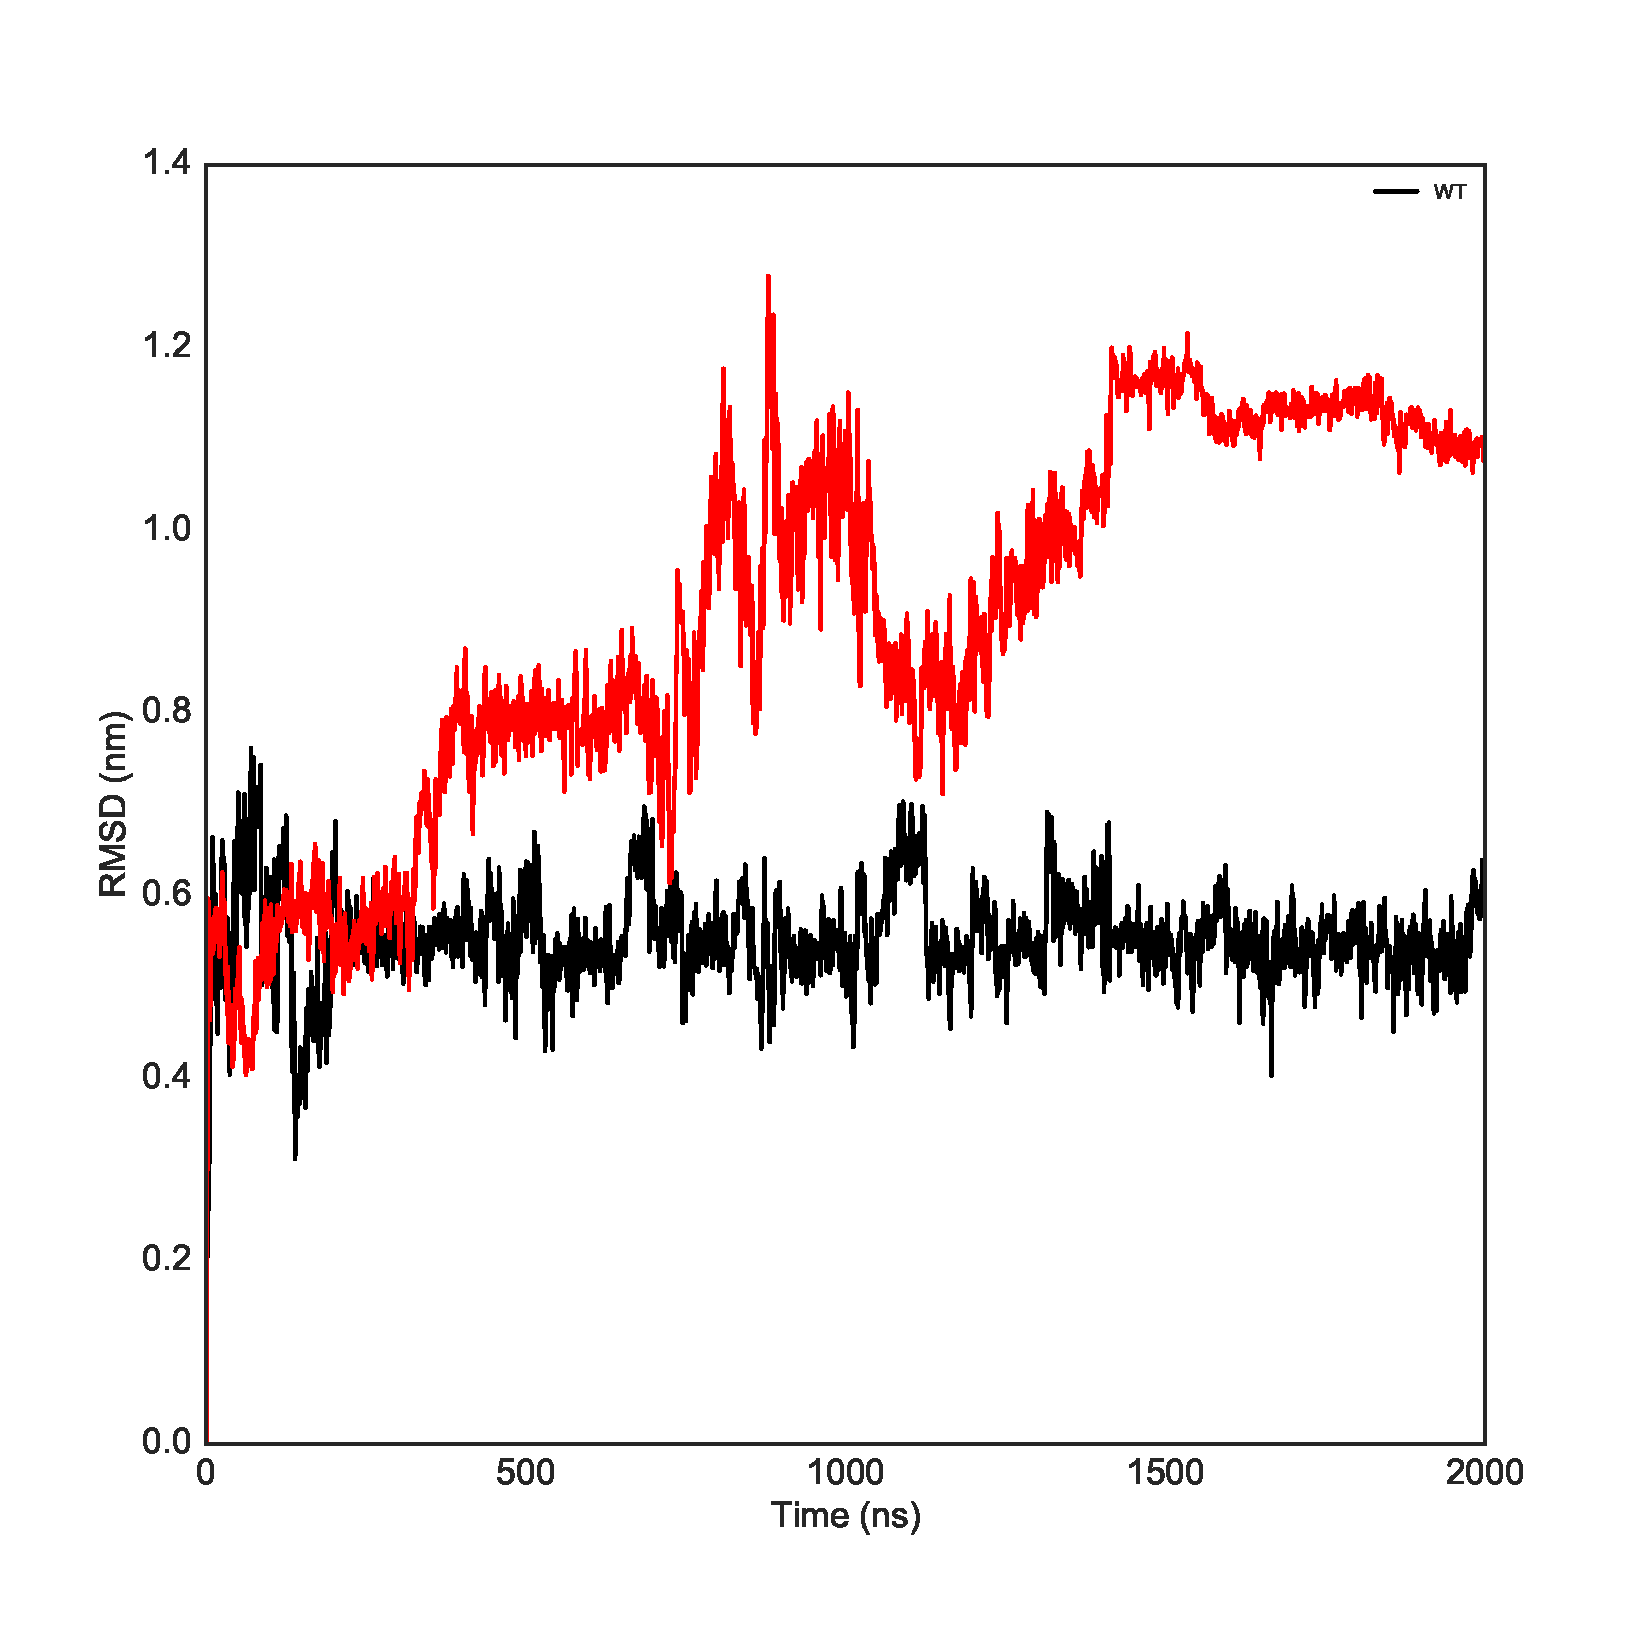
\includegraphics[width=0.49\textwidth]{rmsd}}
	\subfigure[RMSD 10ns window]{\label{fig:rmsd10}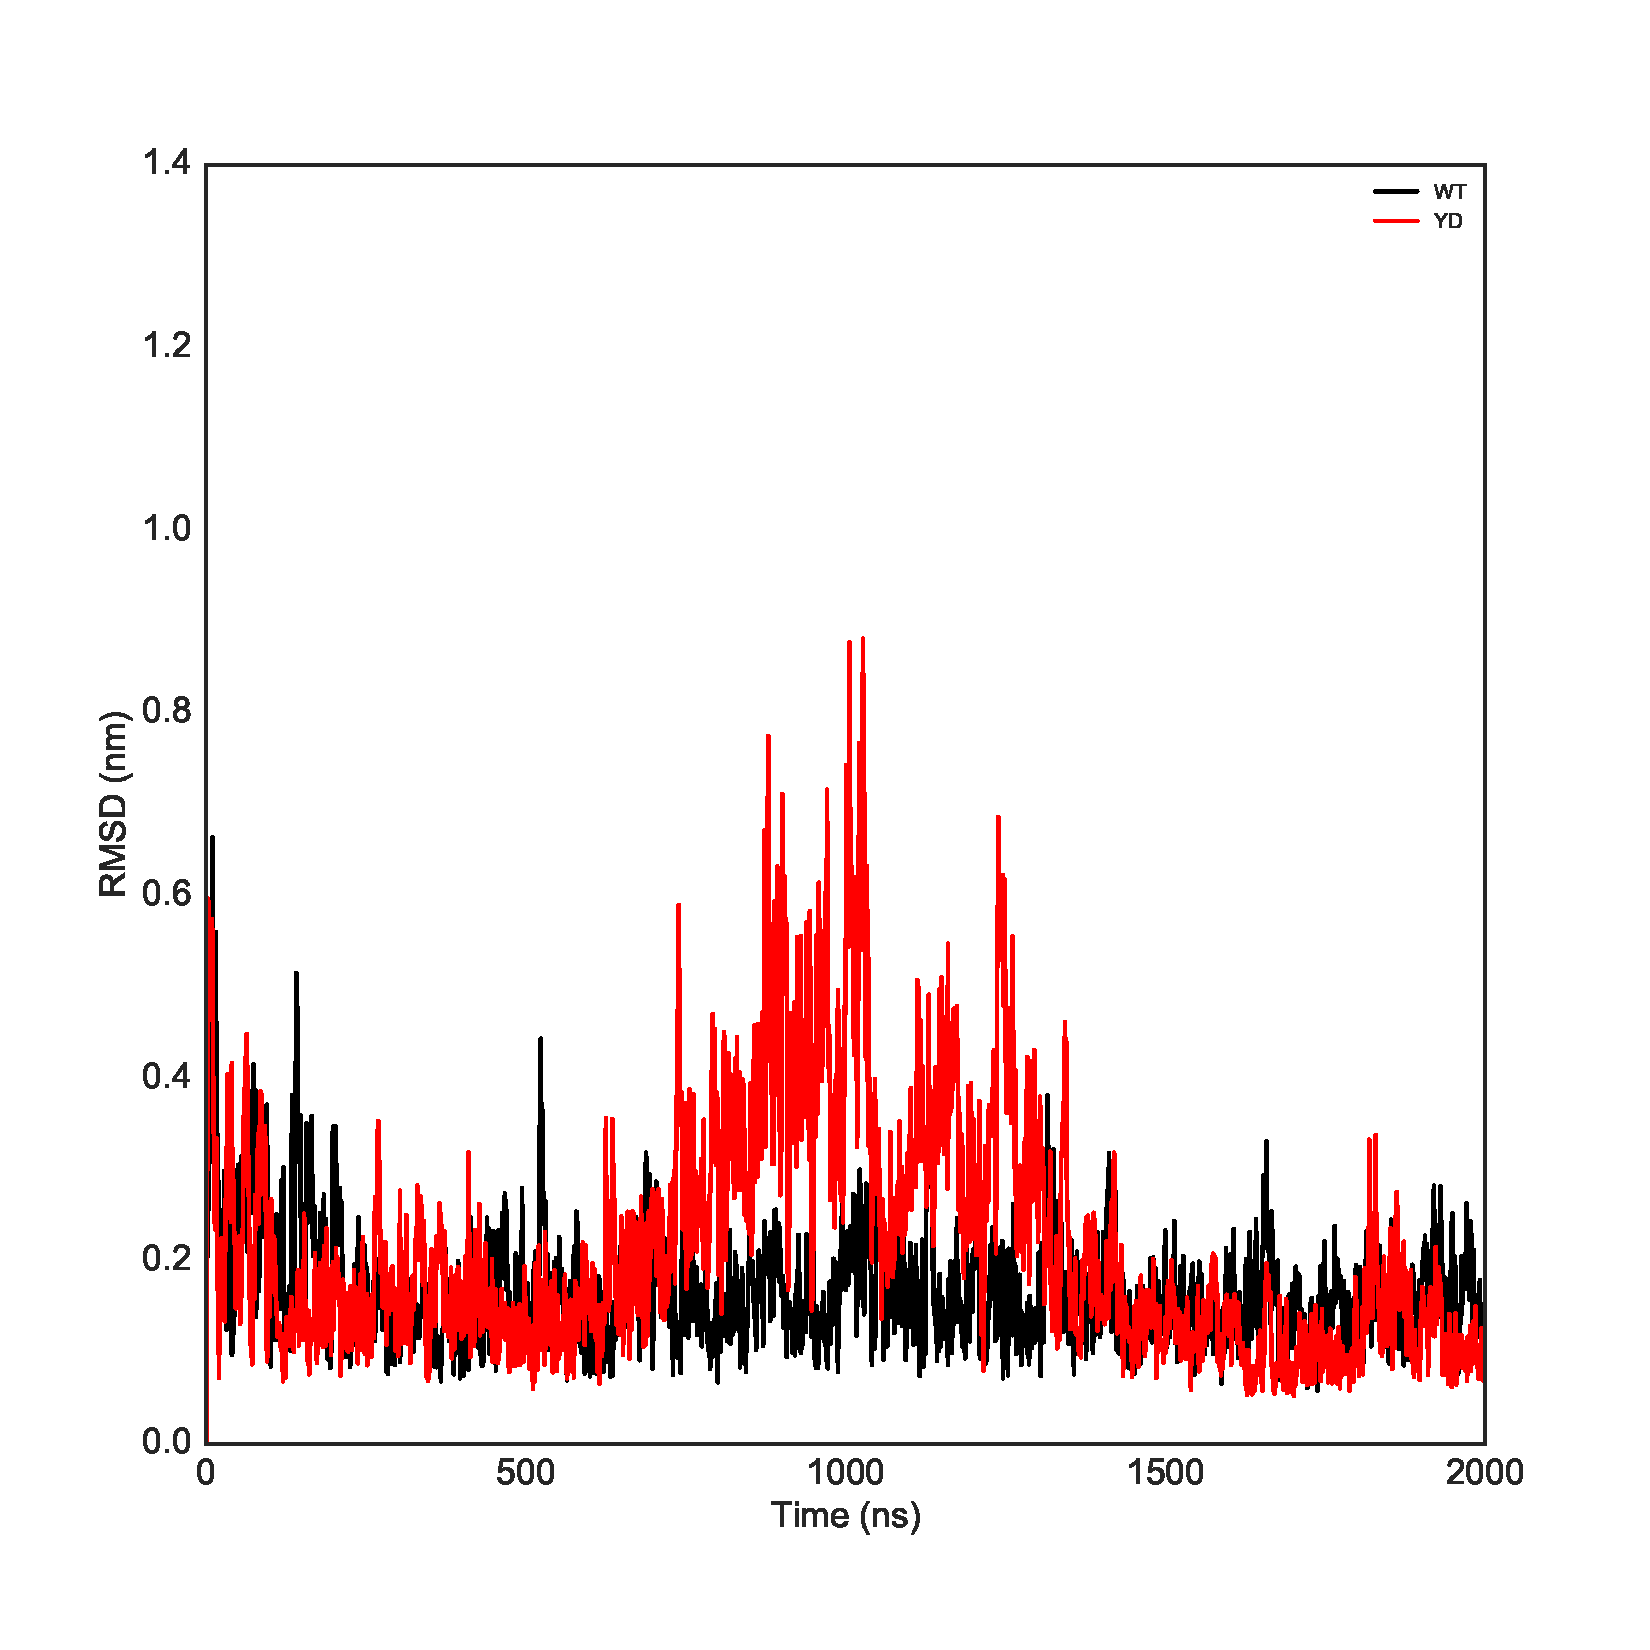
\includegraphics[width=0.49\textwidth]{rmsd_10}}
	\FigureCaption{RMSD}{RMSD plot over simulation time comparing each frame to the starting frame \figref{fig:rmsdinitial} shows YD mutation induces conformational changes absent in WT. 10ns sliding window RMSD plot shows rapid conformational switching in YD simulation in the middle portion of the simulation. \figref{fig:rmsd10}}
	\label{fig:rmsd}
\end{figure}
	
{\it \gct is largely collapsed}

Given that NMR reports transitions between extended and collapsed conformations in the YD mutant, we hypothesize that a similar motion is driving the displacement observed in the RMSD computations. In order to obtain values of compactness that can be compared directly to NMR results, we compute the translational diffusion coefficient (\diffusion) of conformers in our simulations. As a reference point for interpreting the diffusion values of the trajectories, we use the software \texttt{flexiblemeccano} to compute an ensemble of disordered peptides of the YD polypeptide. \texttt{flexiblemeccano} takes a primary sequence as input and generates an ensemble of 3D conformations based on amino acid specific conformational potentials and volume exclusion. We then use \texttt{hydroNMR} to compute \diffusion values for each conformer and obtain a distribution for the \diffusion of the \gct. From this distribution \figref{fig:fm} we obtain a large range of conformations; from highly collapsed, to extended chains against which we can compare MD-derived values.

We computed global averages for the radius of gyration, and translational diffusion coefficient over the \SI{2}{\us} simulations. Both simulations appear to occupy largely collapsed conformations which agrees with experimental findings \figref{fig:dchist}. The WT polypeptide \diffusion mean is \diffusion = \num{1.237e-6} $\pm$ \SI{1.5816e-8}{\dcunits} while the value obtained through NMR is  \diffusion=\num{1.25e-6} $\pm$  \SI{1e-8}{\dcunits}. Similarly to what was seen by NMR, we find that the mean \diffusion of the Y11D \gct polypeptide is slightly lower than that of the WT \gct (\diffusion= \num{1.224e-6} $\pm$ \SI{3.503e-8}{\dcunits}). These results confirm that the \gct, while disordered, is more compact than a fully denatured polypeptide chain, and that the YD \gct is more extended on average.




\begin{figure}
	\centering     %%% not \center
	\subfigure[Distribution of \diffusion in conformer ensemble]{\label{fig:fmdist}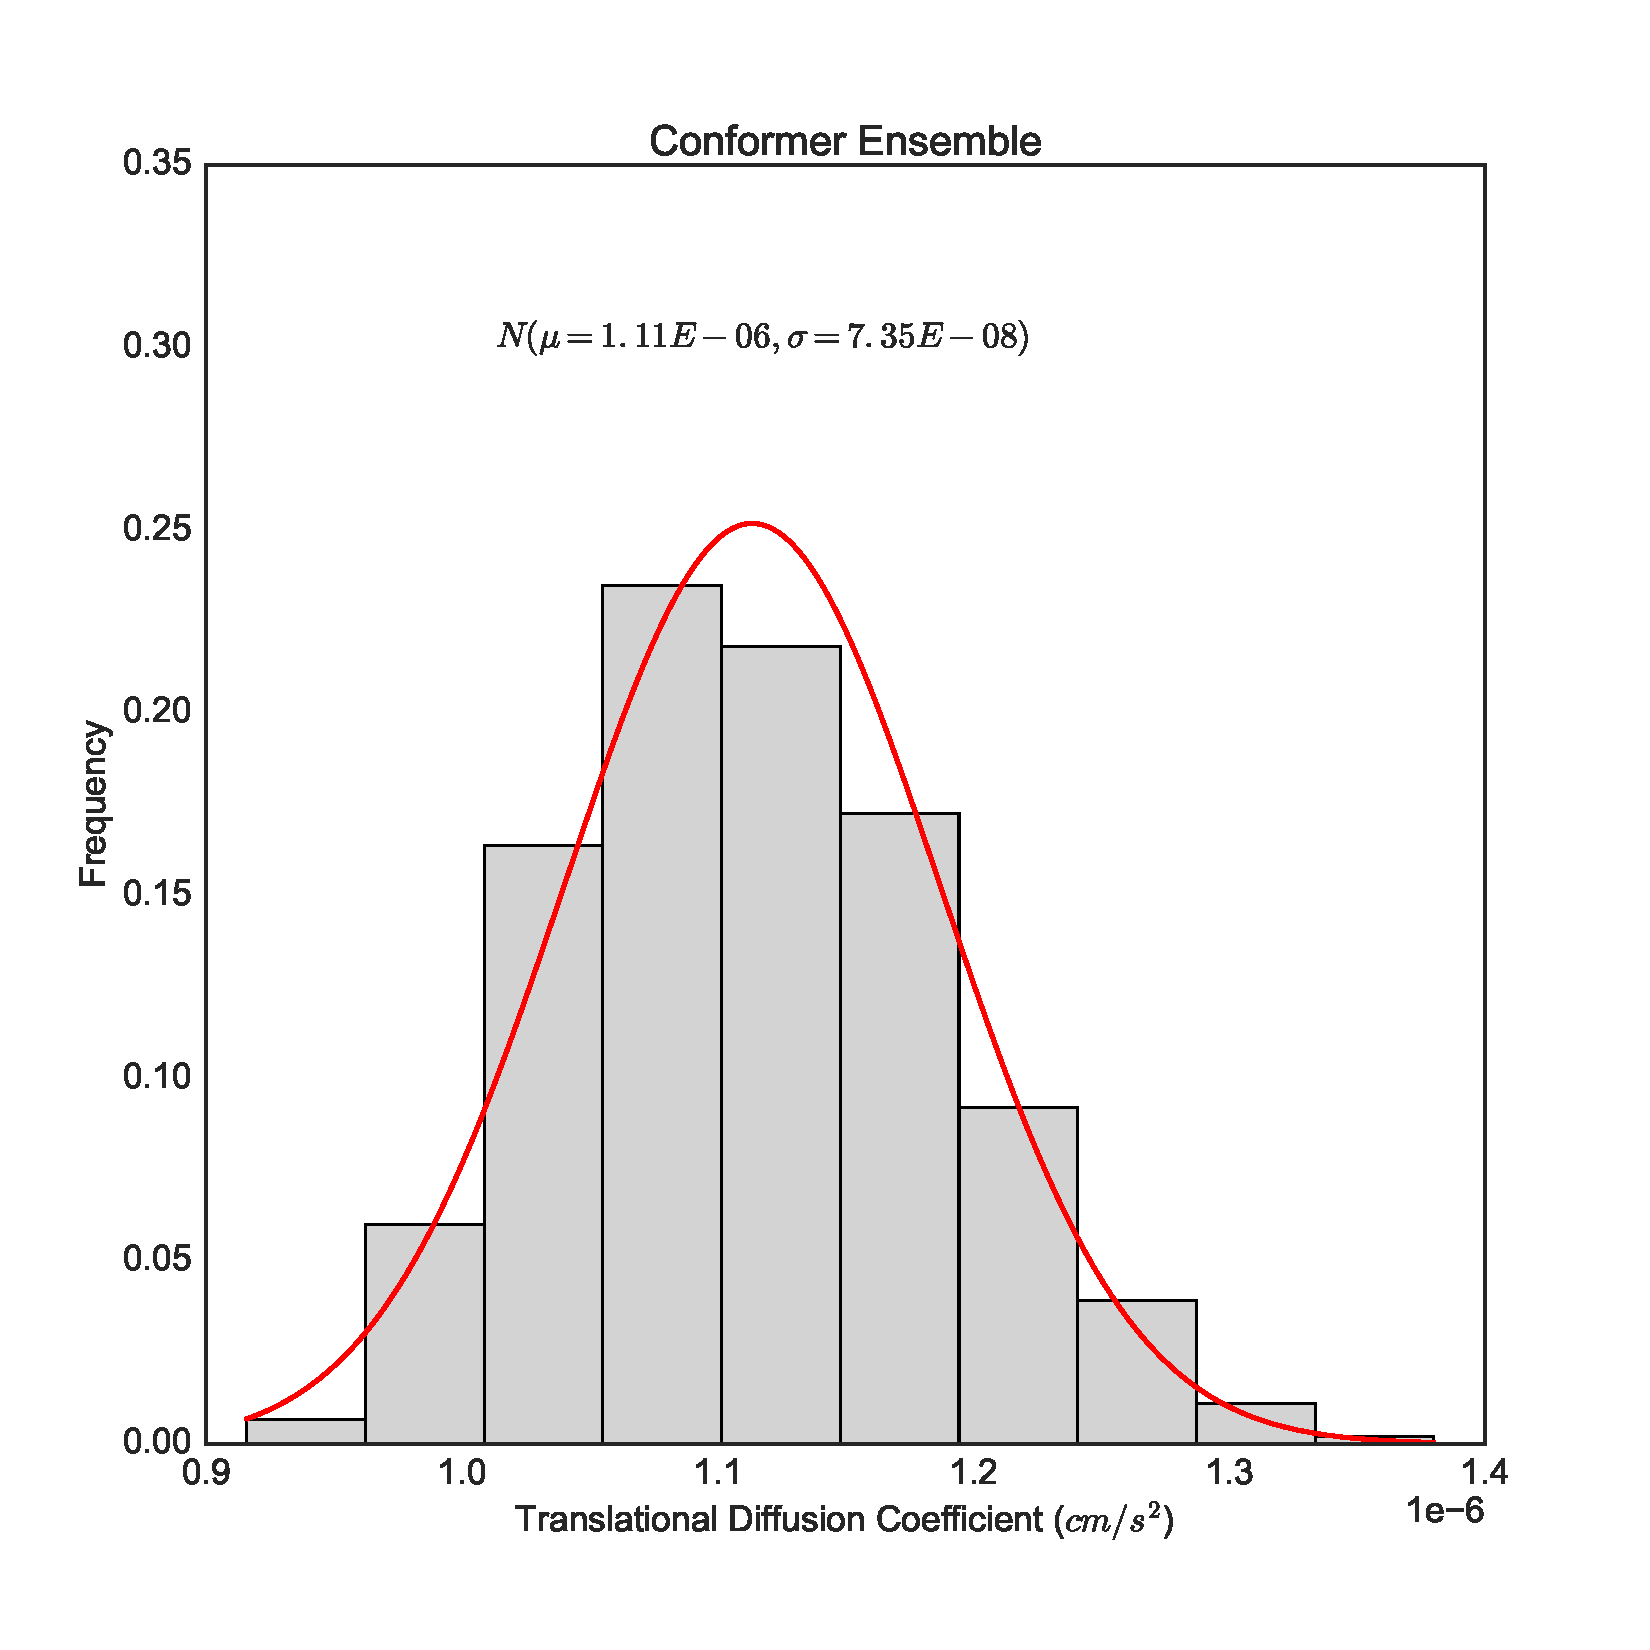
\includegraphics[width=0.49\textwidth]{FM_hist}}
	\subfigure[Representative structures]{\label{fig:rainbows}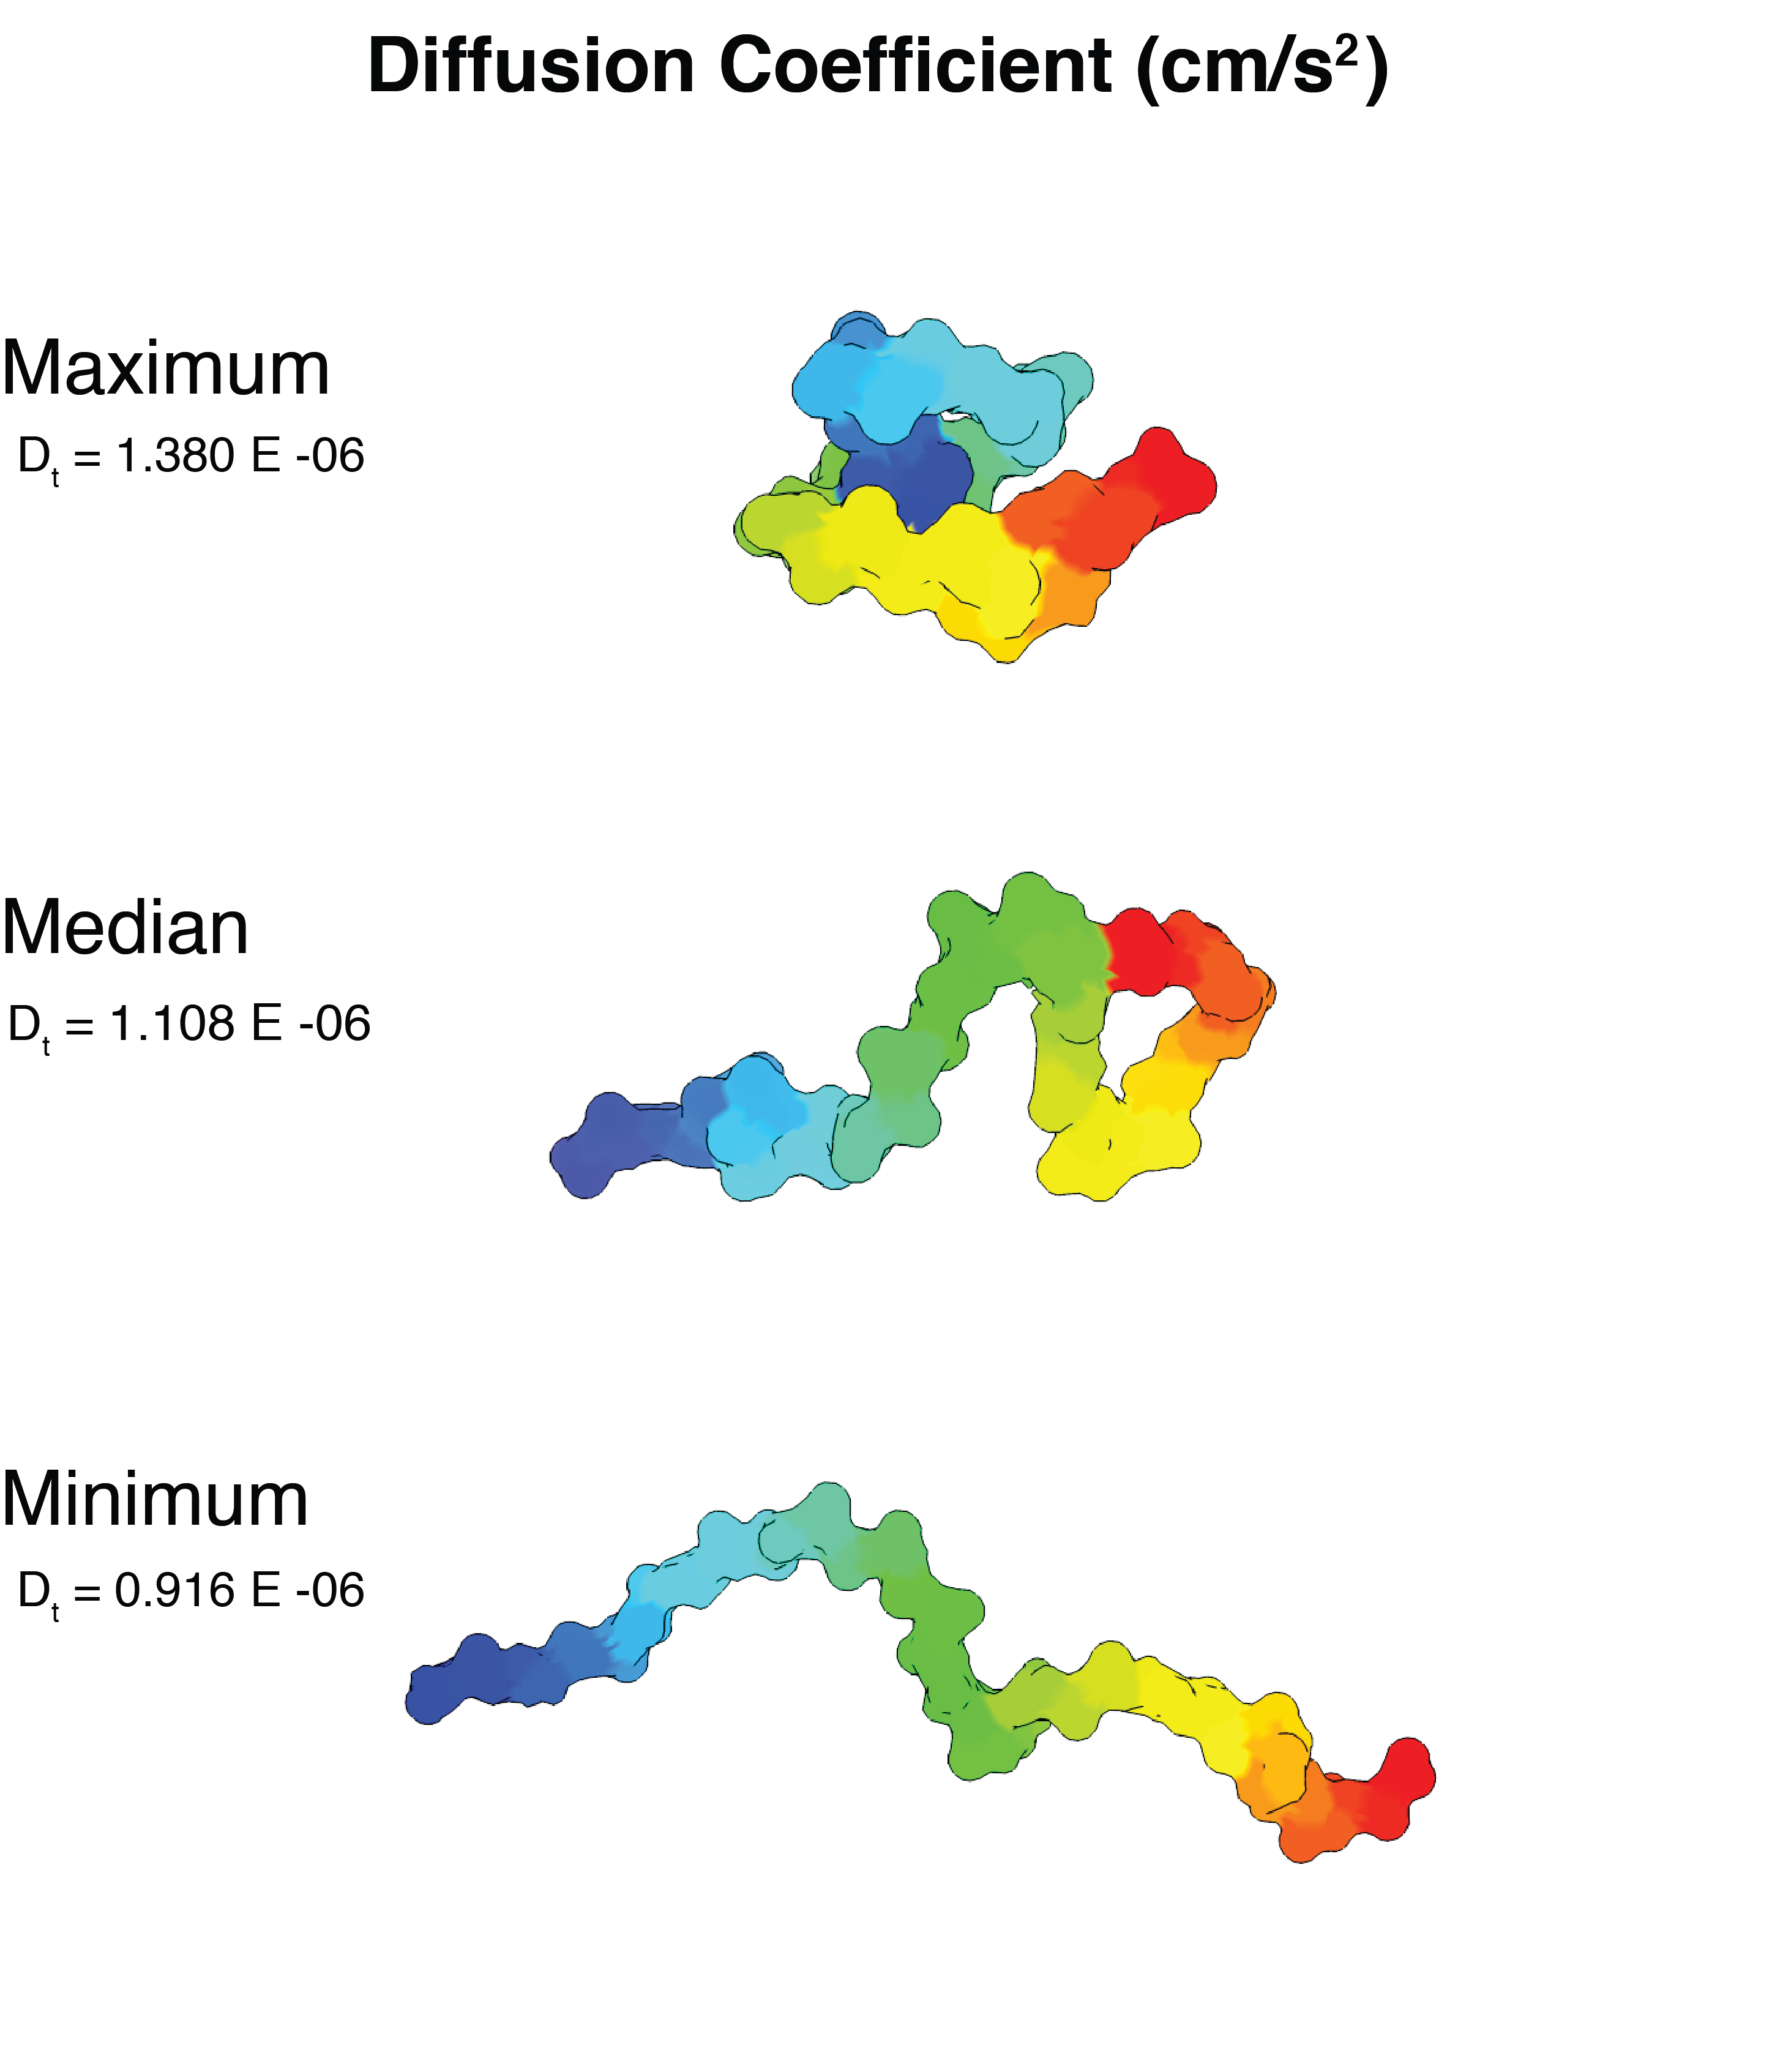
\includegraphics[height=0.35\textheight]{FM_rainbows}}
	\FigureCaption{\gct predicted conformational ensemble}{We use \texttt{flexiblemeccano} to obtain a conformer ensemble based on the primary sequence of the \gct and plot \diffusion for every conformer in the set of 10,000 sampled structures \figref{fig:fmdist}. We visualize the structures corresponding to the maximum, minimum, and median \diffusion. \figref{fig:rainbows}}
	\label{fig:fm}
\end{figure}

Translational diffusion coefficient measurements in NMR report that both \gct forms primarily occupy collapsed conformations. The global experimental average for the WT polypeptide obtained through NMR is \diffusion=\num{1.25e-6} $\pm$  \SI{1e-8}{\dcunits} which agrees well with the NMR-derived value (\diffusion=\num{1.25e-6} $\pm$  \SI{1e-8}{\dcunits}. Similarly to what was seen by NMR, we find that the mean \diffusion of the Y11D \gct polypeptide is slightly lower than that of the WT \gct (\diffusion= \num{1.224e-6} $\pm$ \SI{3.503e-8}{\dcunits}). These results confirm that the \gct, while disordered, is more compact than a fully denatured polypeptide chain \figref{fig:dclines}. 

Although both forms of the \gct primarily occupy collapsed and disordered conformations, we do observe that, as in NMR, the YD \gct has a slightly lower mean \diffusion than WT. From NMR we hypothesize that this is caused by transitions between compacted and extended driven by enhanced dynamics in the YD mutant. Lending support to this hypothesis, we show that we are able to explain the distribution of diffusion coefficients in the YD mutant as the sum of two gaussian distributions with parameters $\mu_1 =\SI{1.24e-6}{\dcunits}, \sigma_2= \num{2.34e-8}, \mu_2 =\SI{1.18e-6}{\dcunits}, \sigma_2= \num{2.21e-8}$ \figref{fig:dchistyd}. This suggests that the YD dynamics likely give rise to a two-state system where a minor state occupies extended conformations \figref{fig:dclines}. Meanwhile, the WT \diffusion distribution is best explained by a single normal distribution which suggests that the peptide occupies a single stable state which corresponds to the compacted portion of conformation space \figref{fig:dchistwt}.

\begin{figure}
\centering     %%% not \center
\subfigure[WT]{\label{fig:dchistwt}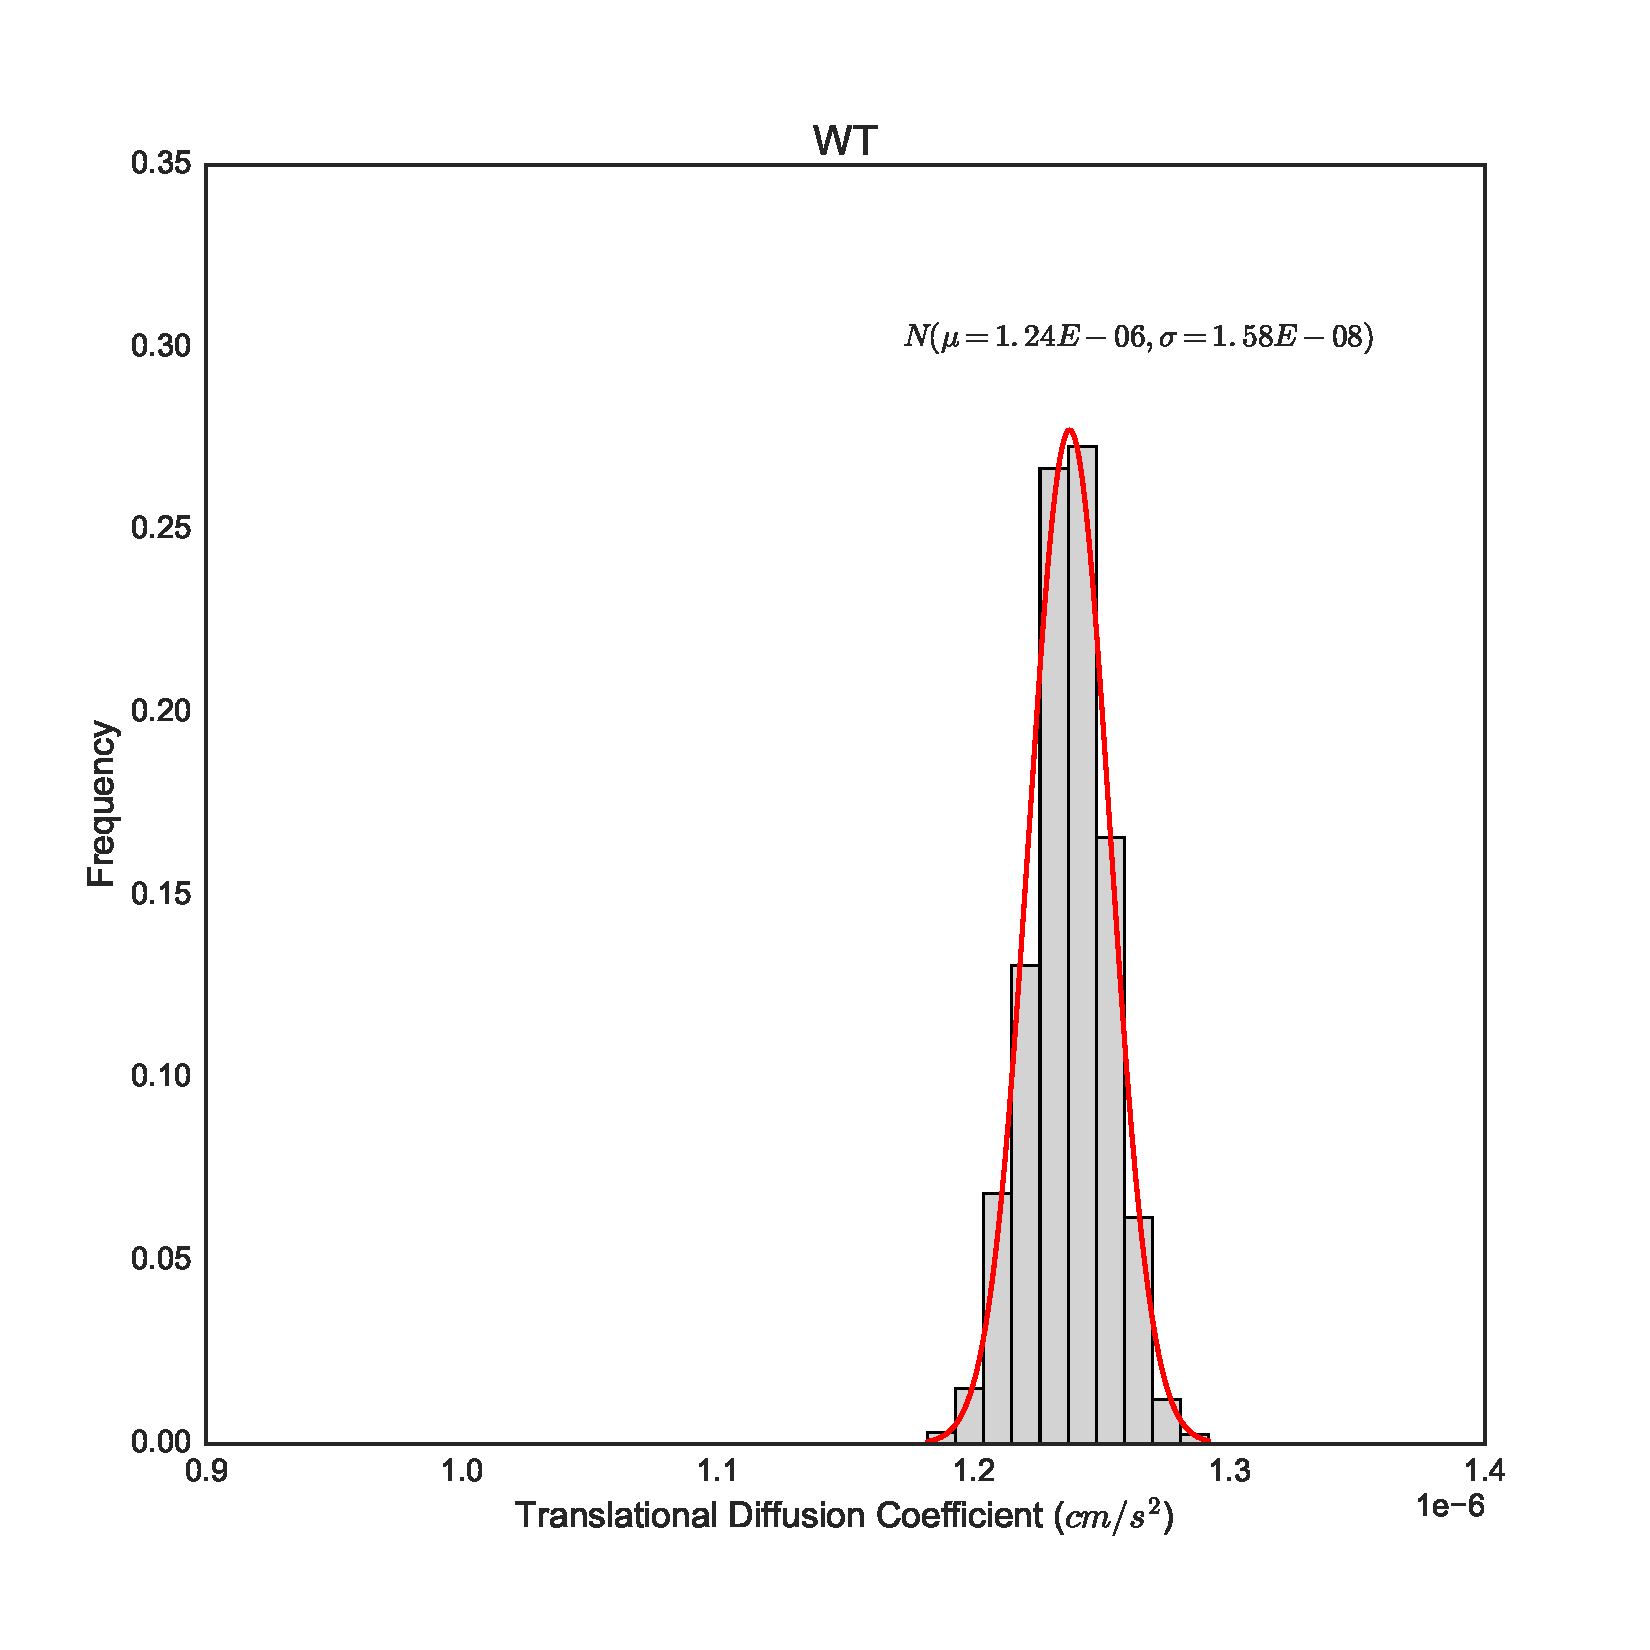
\includegraphics[width=0.49\textwidth]{wt_hist}}
\subfigure[YD]{\label{fig:dchistyd}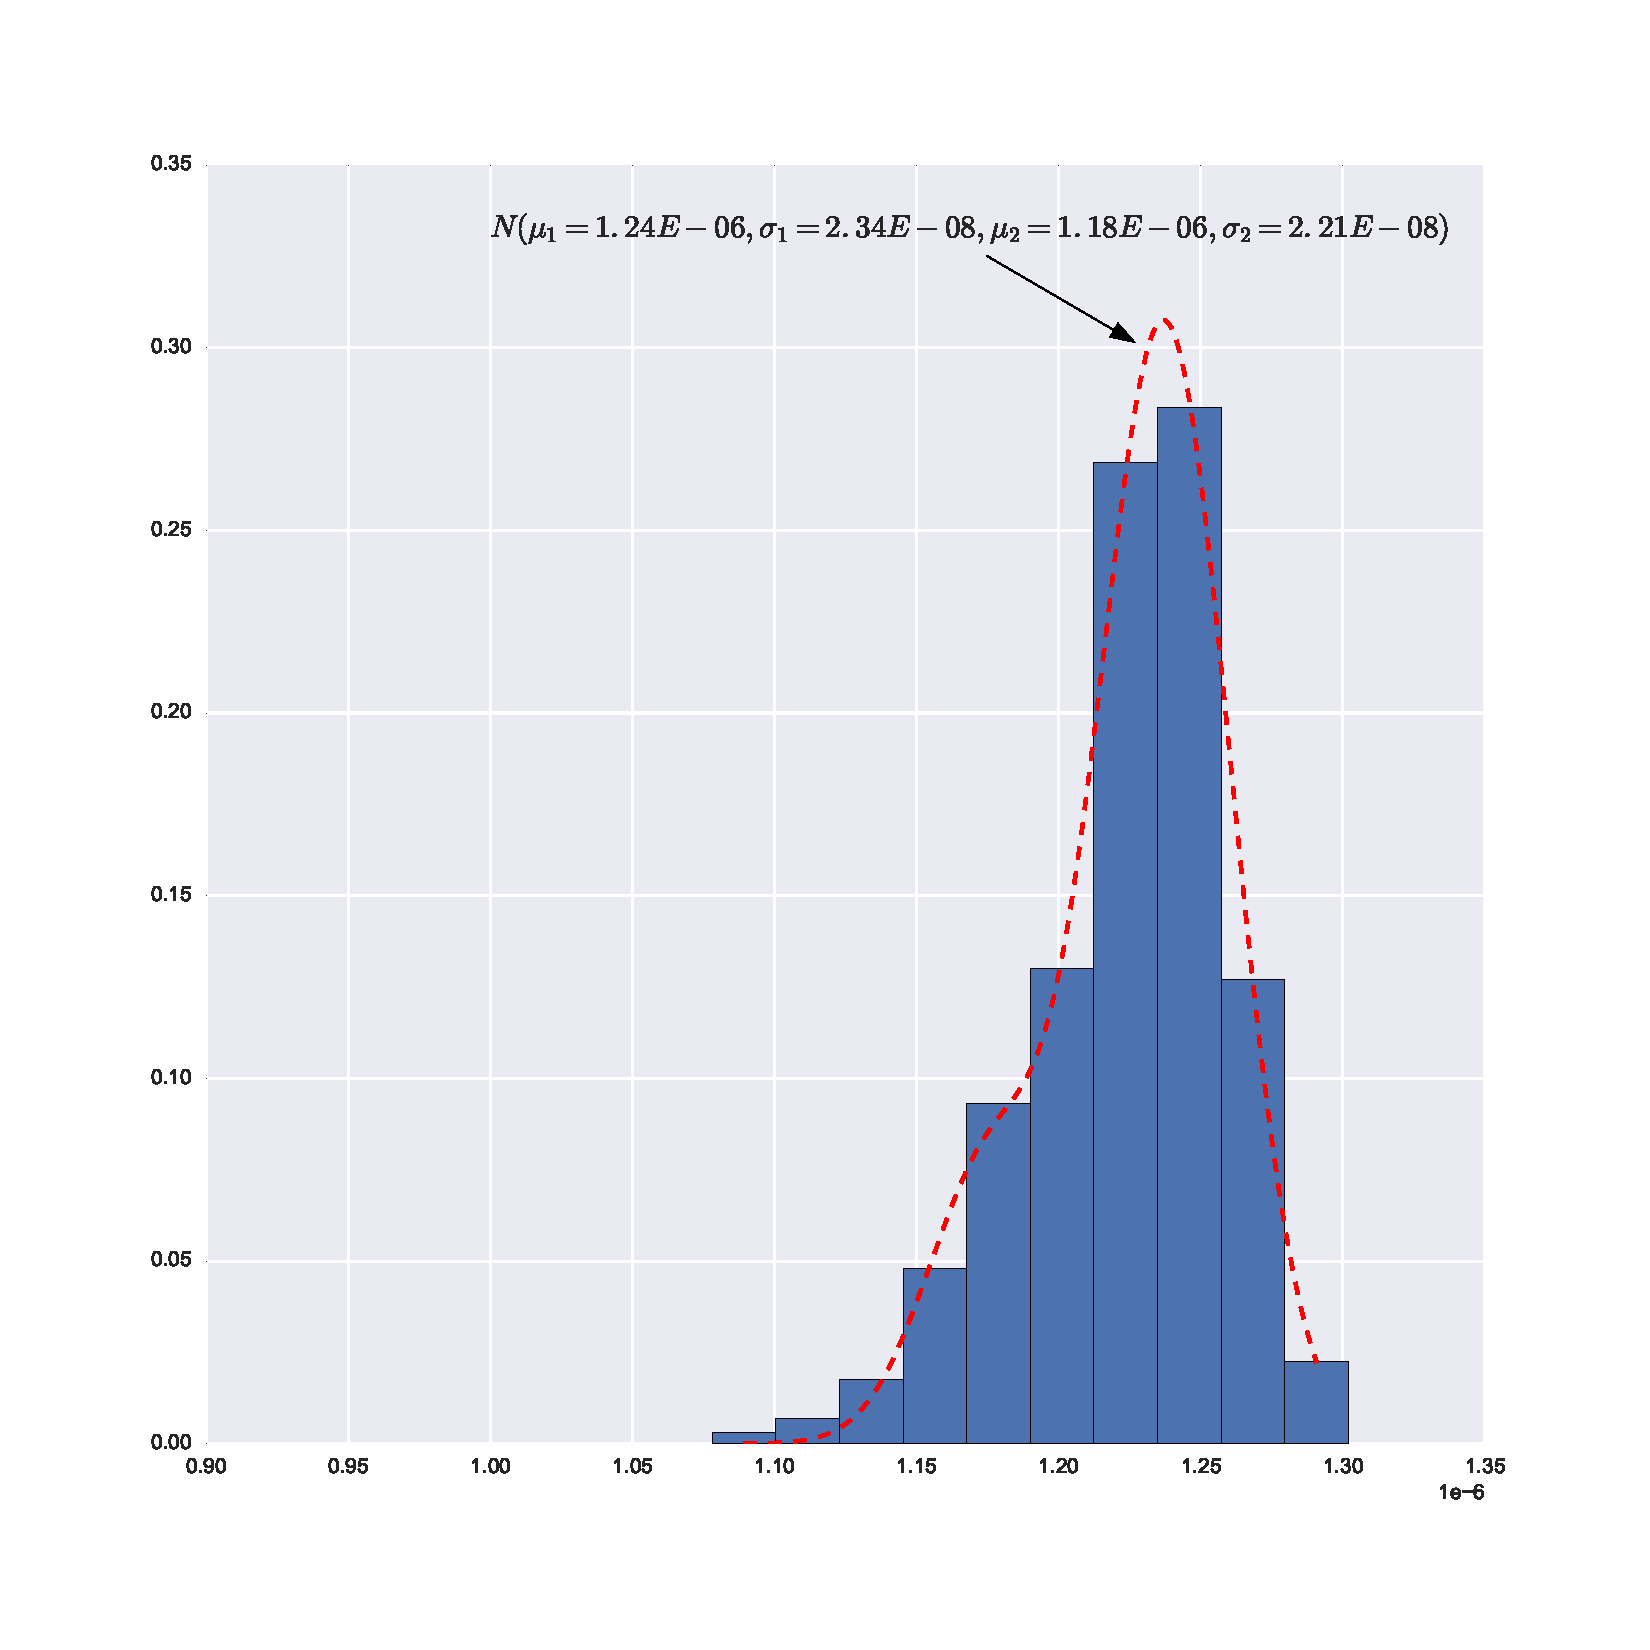
\includegraphics[width=0.49\textwidth]{yd_2gauss}}
\subfigure[Distribution Overlay]{\label{fig:dclines}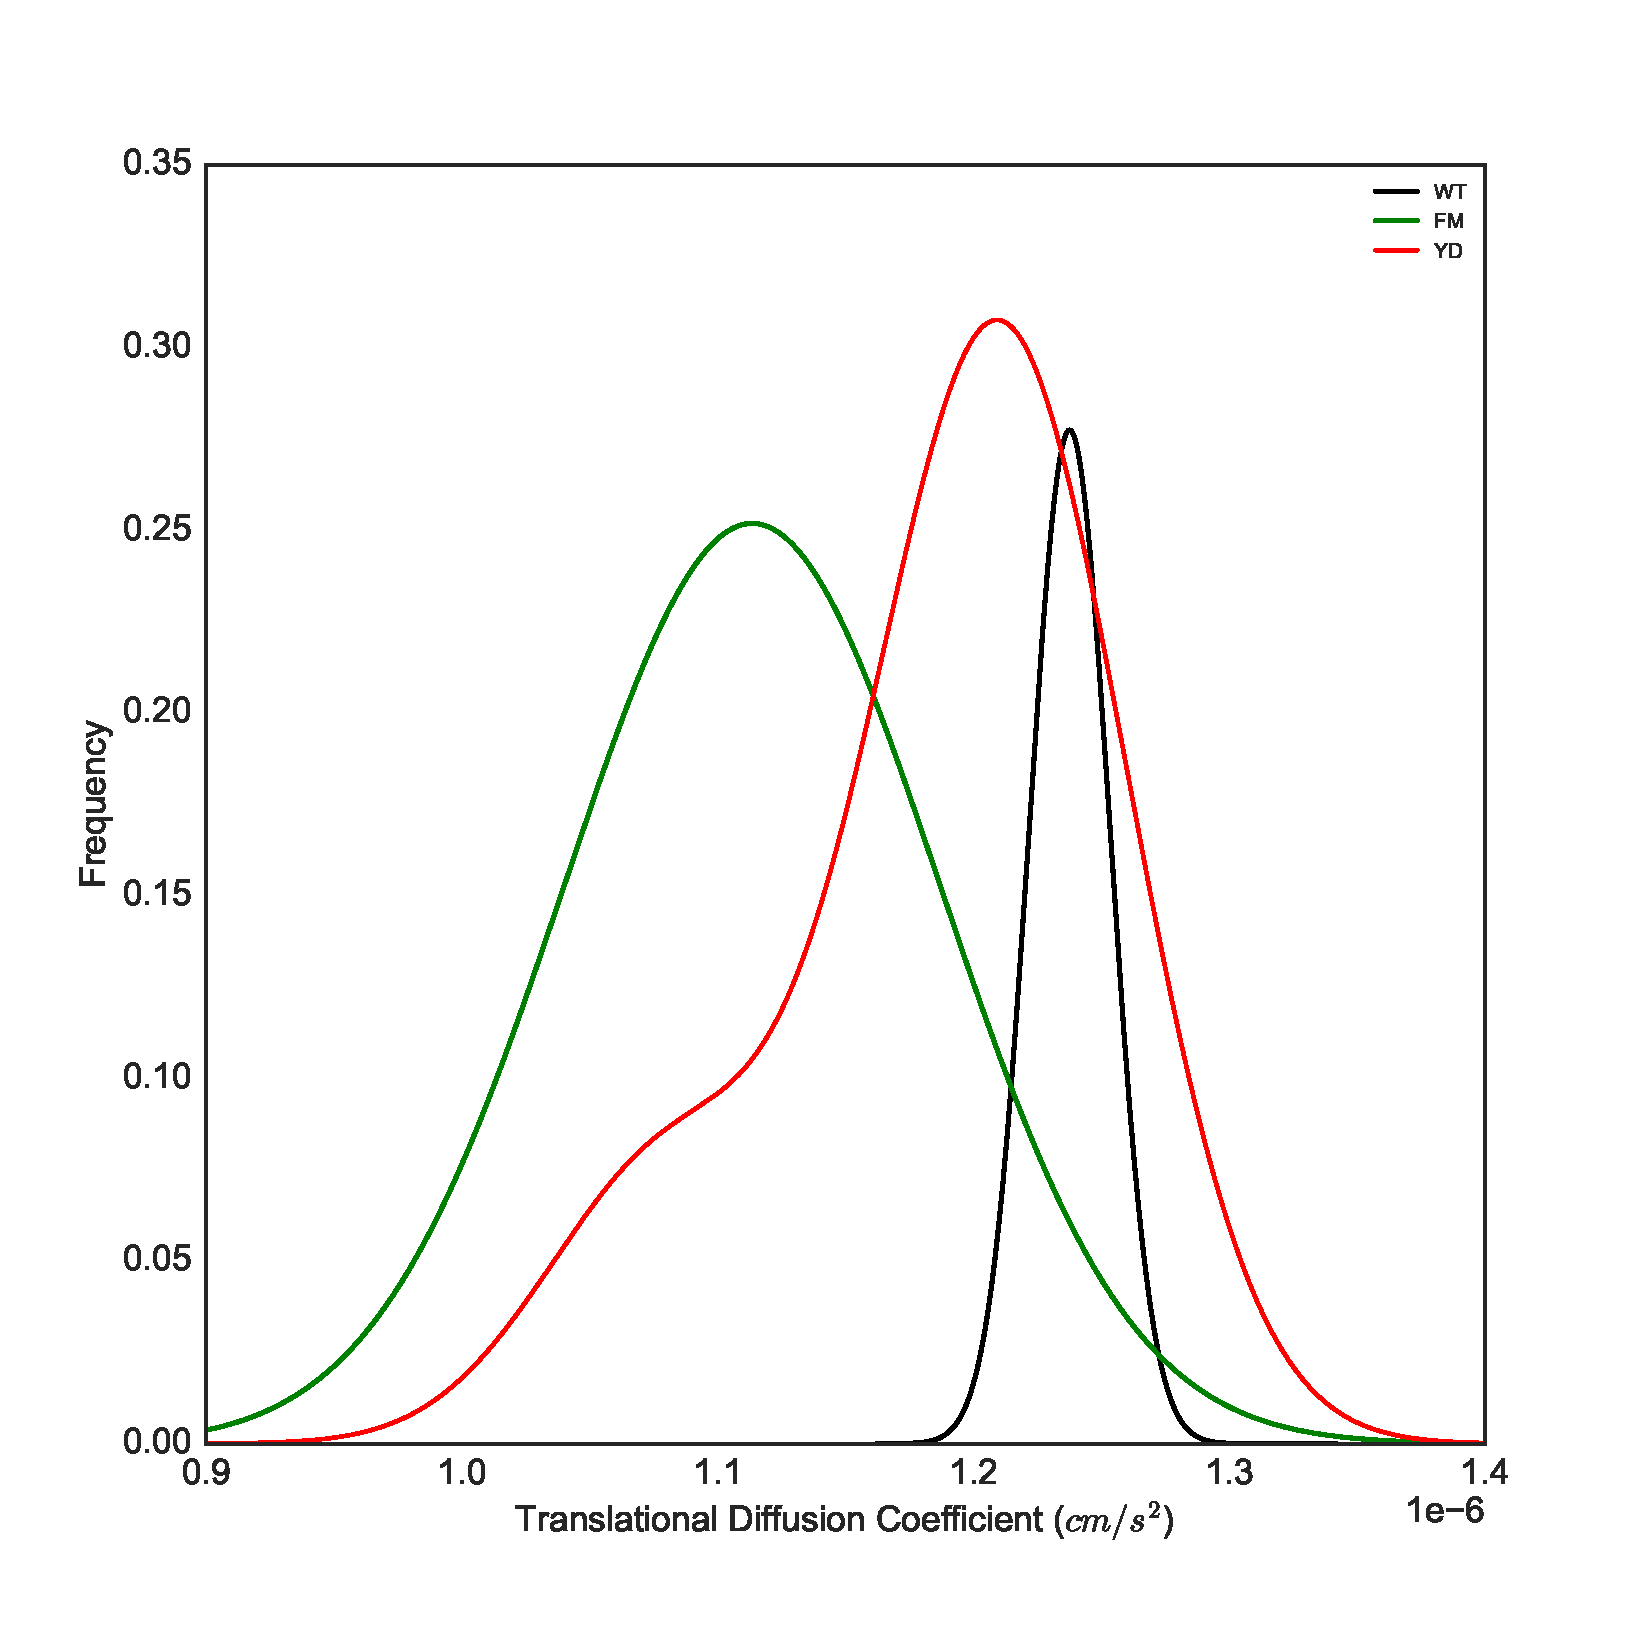
\includegraphics[width=0.49\textwidth]{lines_dc}}
\FigureCaption{Distribution of diffusion coefficients}{Frequency histograms of translational diffusion coefficient for both \gct forms. WT \gct \figref{fig:dchistwt} is closely centered around a compact conformation while the YD mutant also occupies a major collapsed state but also explored a minor extended state \figref{fig:dchistyd}. The resulting distribution of YD can be expressed as the sum of two gaussian distributions, reflecting the two-state nature of the system. \figref{fig:dclines} depicts an overlay of both \gct distributions with the predicted conformational ensemble computed by \texttt{flexiblemeccano} and shows that WT \gct remains in the collapsed region of the ensemble while YD explores more extended regions.}
\label{fig:dchist}
\end{figure}



\begin{figure}
	\centering     %%% not \center
	\subfigure[\diffusion over simulation time]{\label{fig:dctimelines}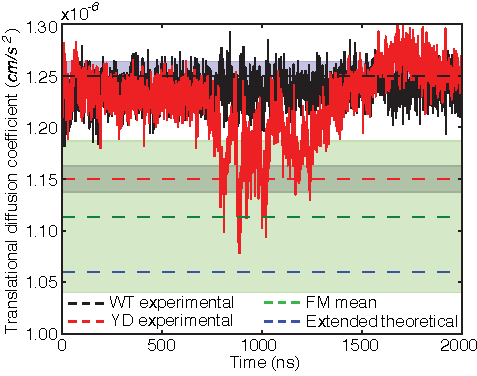
\includegraphics[height=0.35\textheight]{dc_ts}}
	\subfigure[Representative structures]{\label{fig:dctimestructs}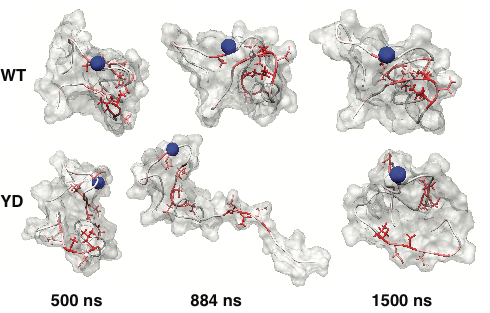
\includegraphics[height=0.3\textheight]{dc_strucs}}
	\FigureCaption{Time series of  conformational sampling of γ−CT under Molecular Dynamics Simulations.}{ \figref{fig:dctimelines} Translational diffusion coefficients of conformations of the WT (black) and Y11D (red) \gct polypetides sampled at \SI{1}{\ns} intervals over a $2 \mu s$ MD simulation (2000 conformations per condition). Experimentally determined \diffusion are shown as a line with the associated error indicated by a shaded region on either side.  The theoretical \diffusion for a denatured 39 residue protein ~\cite{boschitsch2002fast} is indicated by the dashed blue line. The shaded green color shows 1 standard deviation of a randomly generated ensemble of structures that an unfolded WT or Y11D \gct polypeptide can have based on the amino acid-specific conformational potentials and volume exclusion. This region corresponds to partially extended conformations as seen in \figref{fig:fmdist} \figref{fig:dctimestructs} Structures taken from the simulation at \SI{500}, \SI{887} (minimum \diffusion value) and \SI{1500}{\ns} for WT and Y11D \gct polypeptides.}
	\label{fig:dctime}
\end{figure}

Looking at \diffusion as a function of simulation time, we found that the diffusion coefficient (\diffusion) of the WT \gct remains relatively constant throughout the simulation, (\diffusion = \num{1.237e-6} $\pm$ \SI{1.5816e-8}{\dcunits} and agrees well with the NMR-derived value (\diffusion=\num{1.25e-6} $\pm$  \SI{1e-8}{\dcunits}.  Similarly to what was seen by NMR, we find that the mean \diffusion of the Y11D \gct polypeptide is slightly lower than that of the WT \gct (\diffusion= \num{1.224e-6} $\pm$ \SI{3.503e-8}{\dcunits}). These results confirm that the \gct, while disordered, is more compact than a fully denatured polypeptide chain. Interestingly, between \num{762} to \SI{1255}{\ns} in the MDS, the Y11D \gct underwent transient excursions to less compact con-formations with significantly lower diffusion coefficients (mean \diffusion= \num{1.152e-6} $\pm$ \SI{2.0325e-8}{\dcunits}). This sub-population is more extended (i.e. diffuses more slowly) than any conformation sampled by the WT \gct throughout the entire MDS. While the Y11D \gct extended states do not overlap with the conformational ensemble of the WT \gct polypeptides, they do, however, lie close to the extended conformational space for a typical random-coil poly-peptide, as modeled by \texttt{flexiblemeccano} \figref{fig:dctime}.

In order to visualize a non-overlapping subset of conformations to represent extended and collapsed states, we use the \diffusion distributions in \figref{fig:dchist} to select the conformations within the top and bottom 1\% (20 structures each) of the WT \gct and Y11D \gct. In the case of the WT, we do not expect the upper and lower \diffusion subsets to substantially differ, as the WT \gct conformations exhibit fairly homogeneous compactness overall. For Y11D \gct, we expect the upper \diffusion subset to resemble that of the WT \gct, while the lower \diffusion subset is expected to reflect the transient opening process. We plotted the mean distance between alpha carbons of all pairs of residues as contact maps for the set of collapsed (upper) and extended (lower) conformations of the WT \gct polypeptide \figref{fig:wt_contacts} and the Y11D \gct polypeptide \figref{fig:yd_contacts}.   As expected, the upper and lower \diffusion subsets of the WT \gct and the upper Ds subset of the YD \gct polypeptides show similar patterns of pair-wise contacts.  In contrast, the C-terminal residues in the lower \diffusion subset of the Y11D \gct lose the majority of contacts with N terminal residues, as a consequence of the conformational expansion. Next, we isolated the three conformations from the upper and lower \diffusion subsets of  Y11D \gct poly-peptides with the lowest all-to-all RMS, also known as centroid structures, shown in \figref{fig:representatives} with large relaxation dispersion magnitudes indicated in red. This analysis shows that the extended conformations consist of a compact N-terminus with residues located in the C-terminal region of the \gct, (including dynamically-broadened residues L30, A32 and G34) isolated from the N-terminus and solvent-accessible. Through MD we are able to re-produce the anomalously rapid diffusion (i.e. high compactness) of the WT and Y11D ground-state \gct polypeptides. Moreover, we saw that the YD substitution caused relatively slow collective motions of the entire polypeptide chain, as observed by NMR. This serves as a possible explanation for how residues throughout a disordered polypeptide can experience concerted, two-state, dynamical behaviour in the presence of the Y11D mutation. More specifically, it is the separation of a cluster of residues located in N and C termini of the \gct polypeptide that drives a transition to extended conformations with a concomitant  reduction of the translational diffusion coefficient.


\begin{figure}
\centering     %%% not \center
\subfigure[WT]{\label{fig:wt_contacts}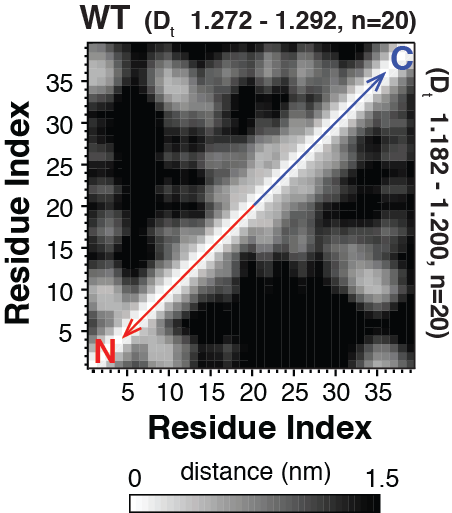
\includegraphics[height=0.35\textheight]{wt_contacts}}
\subfigure[YD]{\label{fig:yd_contacts}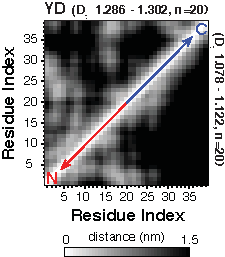
\includegraphics[height=0.35\textheight]{yd_contacts}}
\subfigure[Representative Structures]{\label{fig:representatives}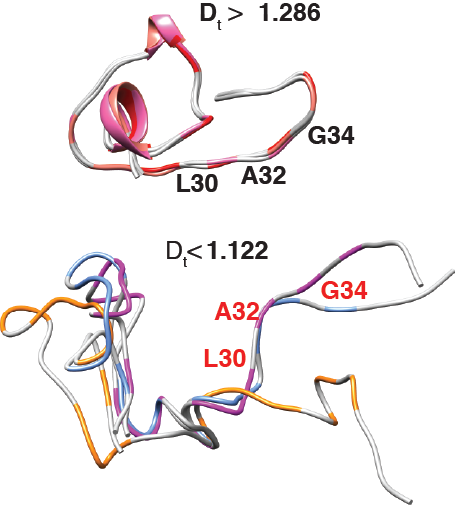
\includegraphics[height=0.35\textheight]{representatives}}
\FigureCaption{Distribution of diffusion coefficients}{All-to-all residue carbon-α distances in structures with lowest 1\% \diffusion  (upper triangle) and highest 1\% \diffusion (lower triangle). Comparison is shown for WT \figref{fig:wt_contacts} and Y11D \figref{fig:yd_contacts} simulations. Representative structures obtained identifying structures with lowest all-to-all RMSD values for the Y11D low diffusion coefficient group. High dispersion residues with $\Delta$R2 values greater than $5 s^{-1}$ are labeled in red.}

\label{fig:contacts}
\end{figure}


\subsection{Collective motions correspond to transitions between extended and collapsed conformations}

Until this point, we have identified the presence of an extended sub-population of the YD \gct that is absent in the WT. This lends support to the hypothesis that the shift in \diffusion measured by NMR is due to transient expansions of the YD backbone into an extended state. Complementary to this finding, is the fact that residues in the YD polypeptide show evidence of collective motions detected as shifts in chemical environment through NMR. This suggests that the transition between states occurs in a coordinated manner. We therefore seek to test whether correlated motions are also present in the simulation, and if they are, whether they can explain the transitions between collapsed and extended states.

We performed covariance analysis, also known as Principal Component Analysis on \gct trajectories to identify major modes of correlated motion in our trajectories. We use \texttt{covar} and \texttt{anaeig} from the \texttt{GROMACS} package to build a backbone atom covariance matrix, extract principal modes, and perform dimensionality reductions through eigenvector projections. In order to eliminate rotational and diffusive  translations which do not correspond to conformational motions, we align all frames in the trajectory to the average structure as computed by \texttt{covar} using RMSD based clustering. As is typical with molecular simulations which operate on a limited number of degrees of freedom, the first few eigenvectors in both trajectories account for nearly all of the variation in the trajectories \figref{fig:eigenvalues}. 

\begin{figure}
\centering
	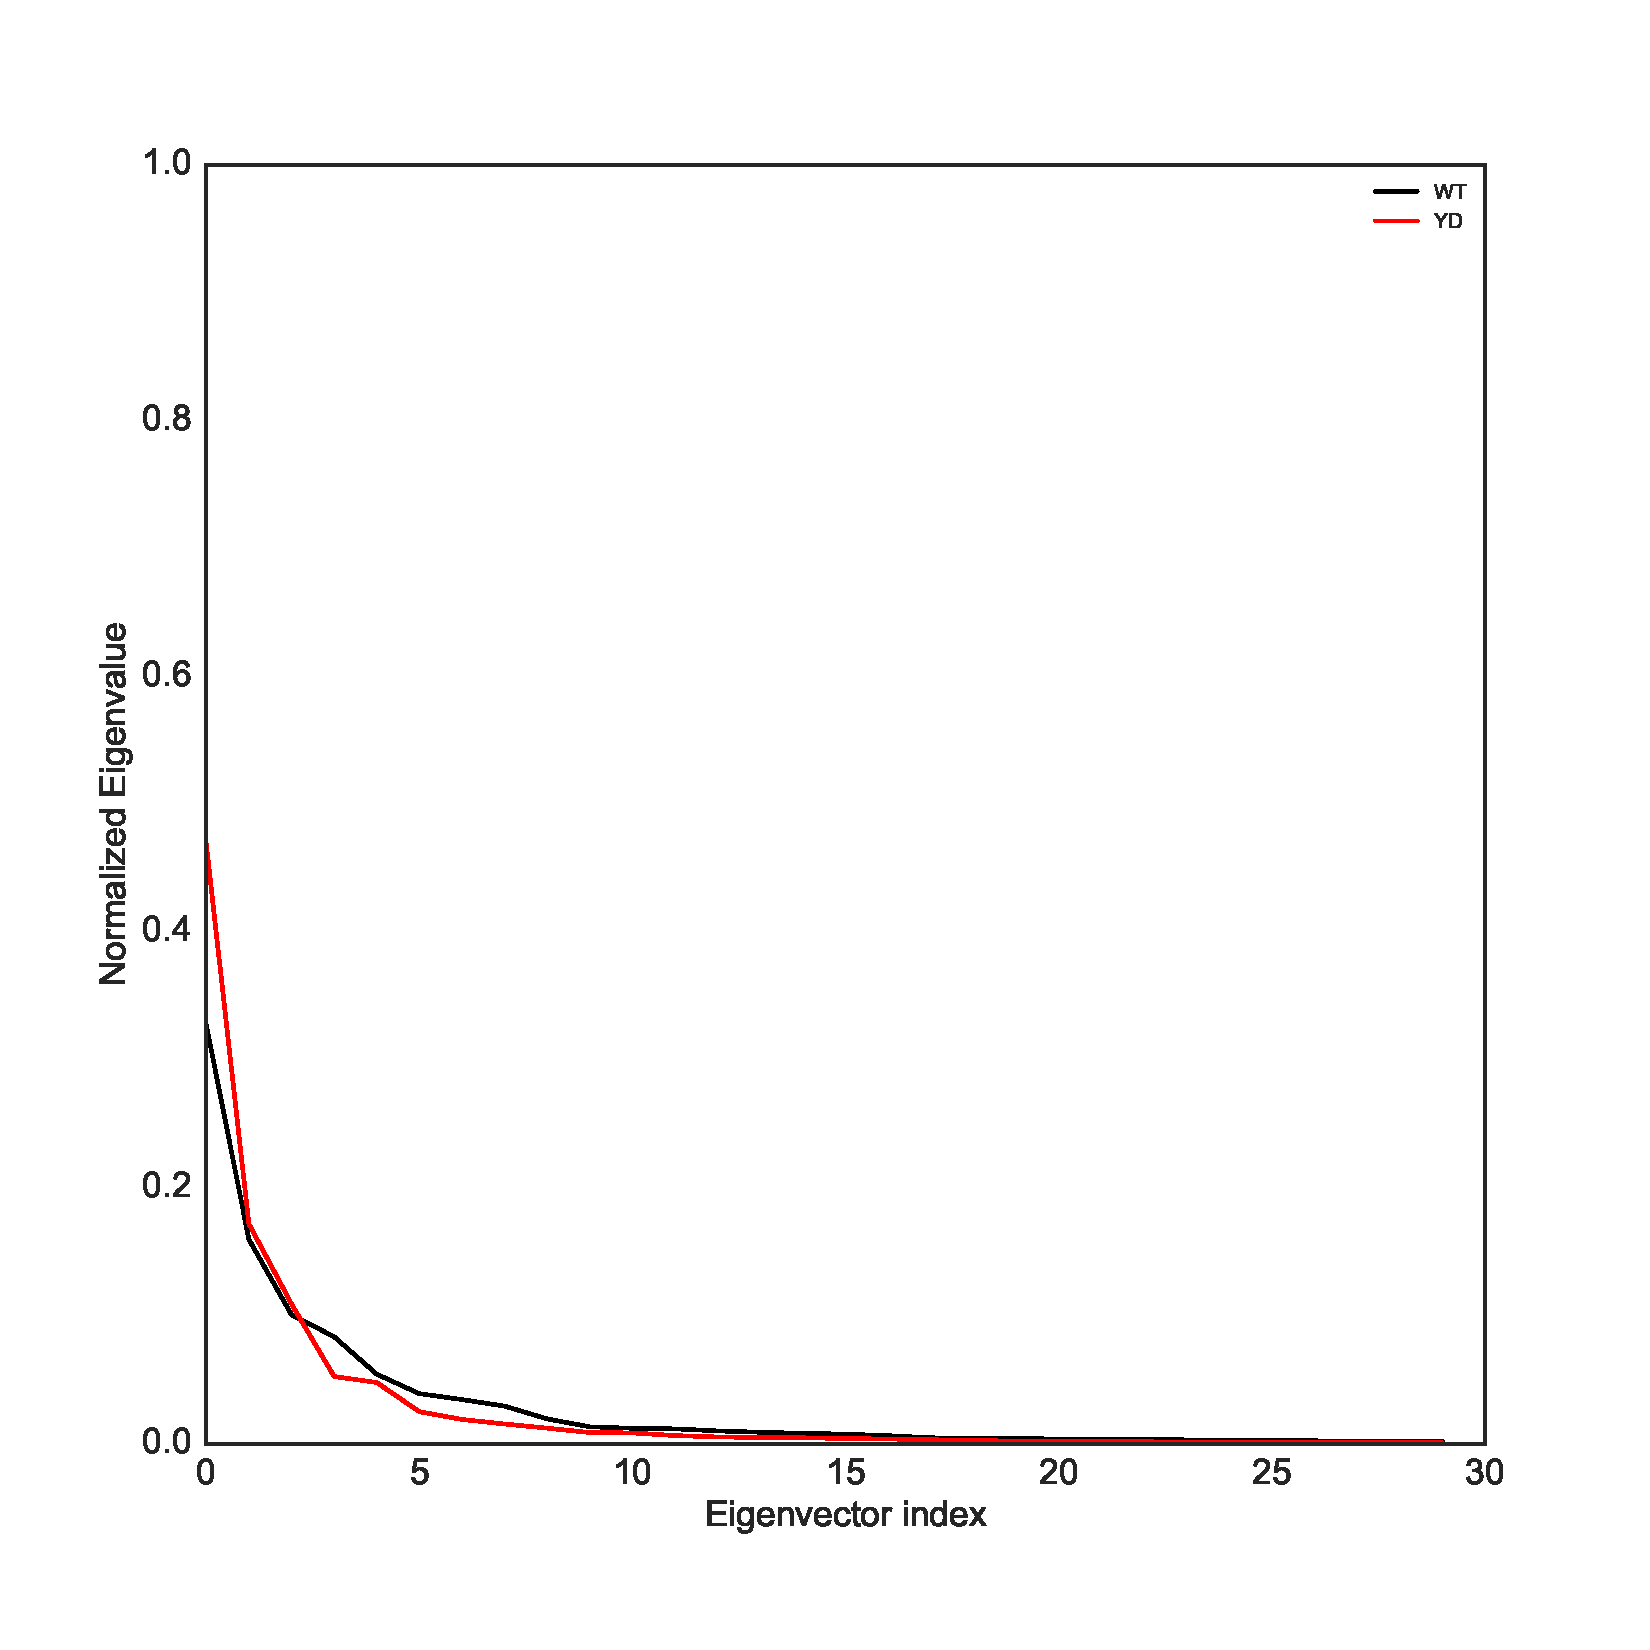
\includegraphics[height=0.35\textheight]{eigenvals}
	\FigureCaption{Eigenvalues of \gct PCA}{Normalized eigenvalues of first 50 eigenvectors resulting from covariance matrix diagonalization of WT and YD trajectories. }
	\label{fig:eigenvalues}
\end{figure}


We therefore focus our attention on the two first major modes of motion. \figref{fig:pca} shows a 2 dimensional projection onto the first two eigenvalues of WT and YD trajectories. Each point represents a 3D conformation in the \SI{2}{\us} simulation projected along the first two eigenvectors. The WT projection shows a conformational space that is closely clustered, indicative of constrained motions consistent with the low dispersions found in NMR, and the single state behaviour suggested by RMSD and \diffusion analysis. However, the YD appears to be exploring  multiple conformation clusters which is in agreement with the presence of high dispersion groups found in NMR. Furthermore, by coloring each conformation with a normalized \diffusion value we are able to show that correlated motions along the major modes correspond with transitions between collapsed and extended states. 

\begin{figure}
	\thispagestyle{empty}
	\centering     %%% not \center
	\subfigure[WT]{\label{fig:wtscatter}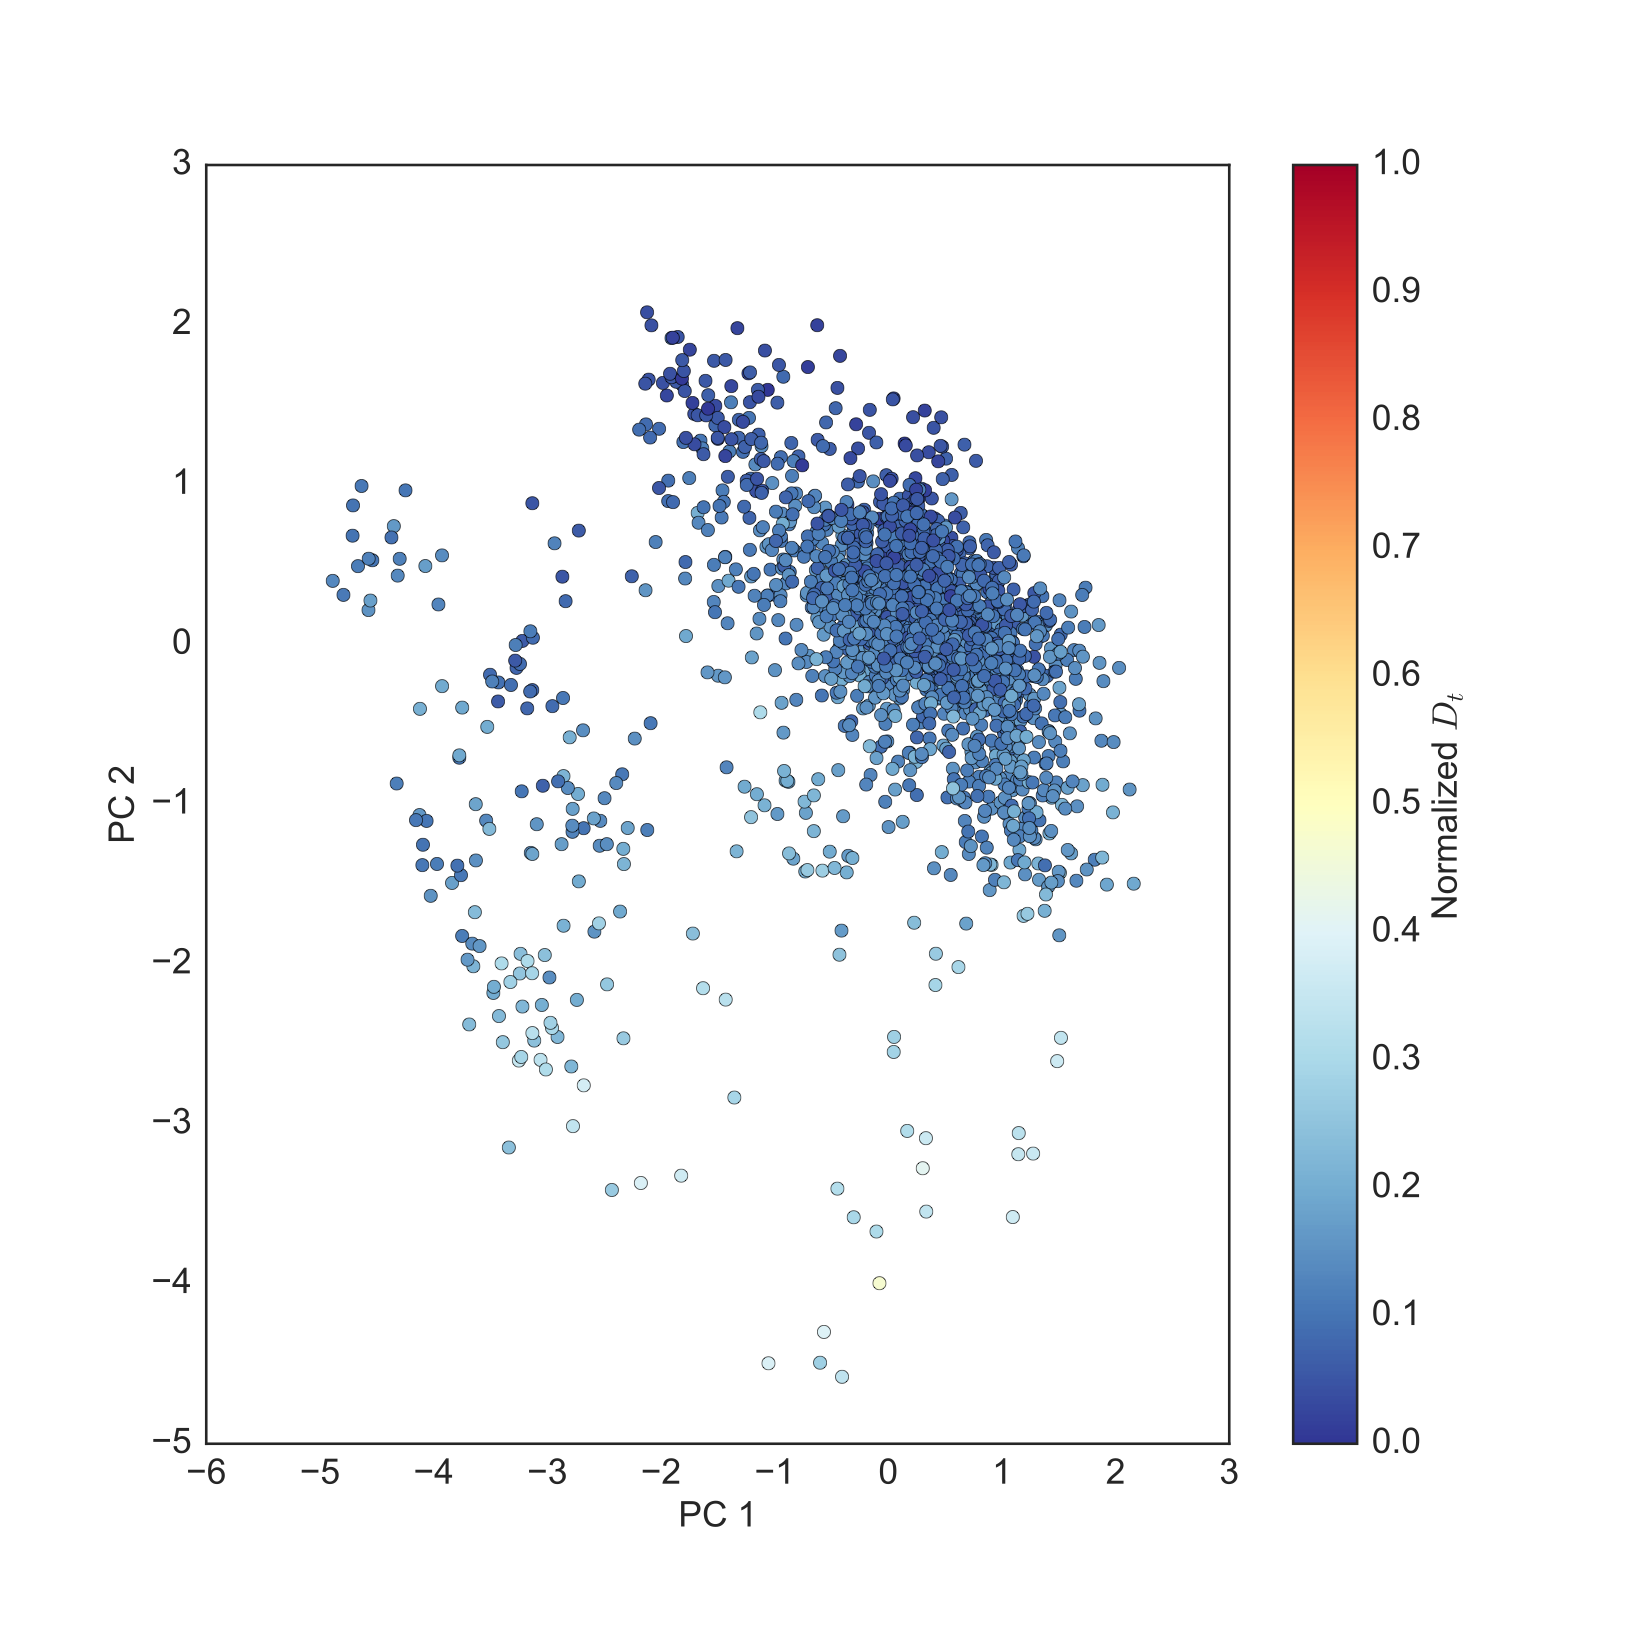
\includegraphics[width=0.49\textwidth]{2d_scatter_wt}}
	\subfigure[YD]{\label{fig:ydscatter}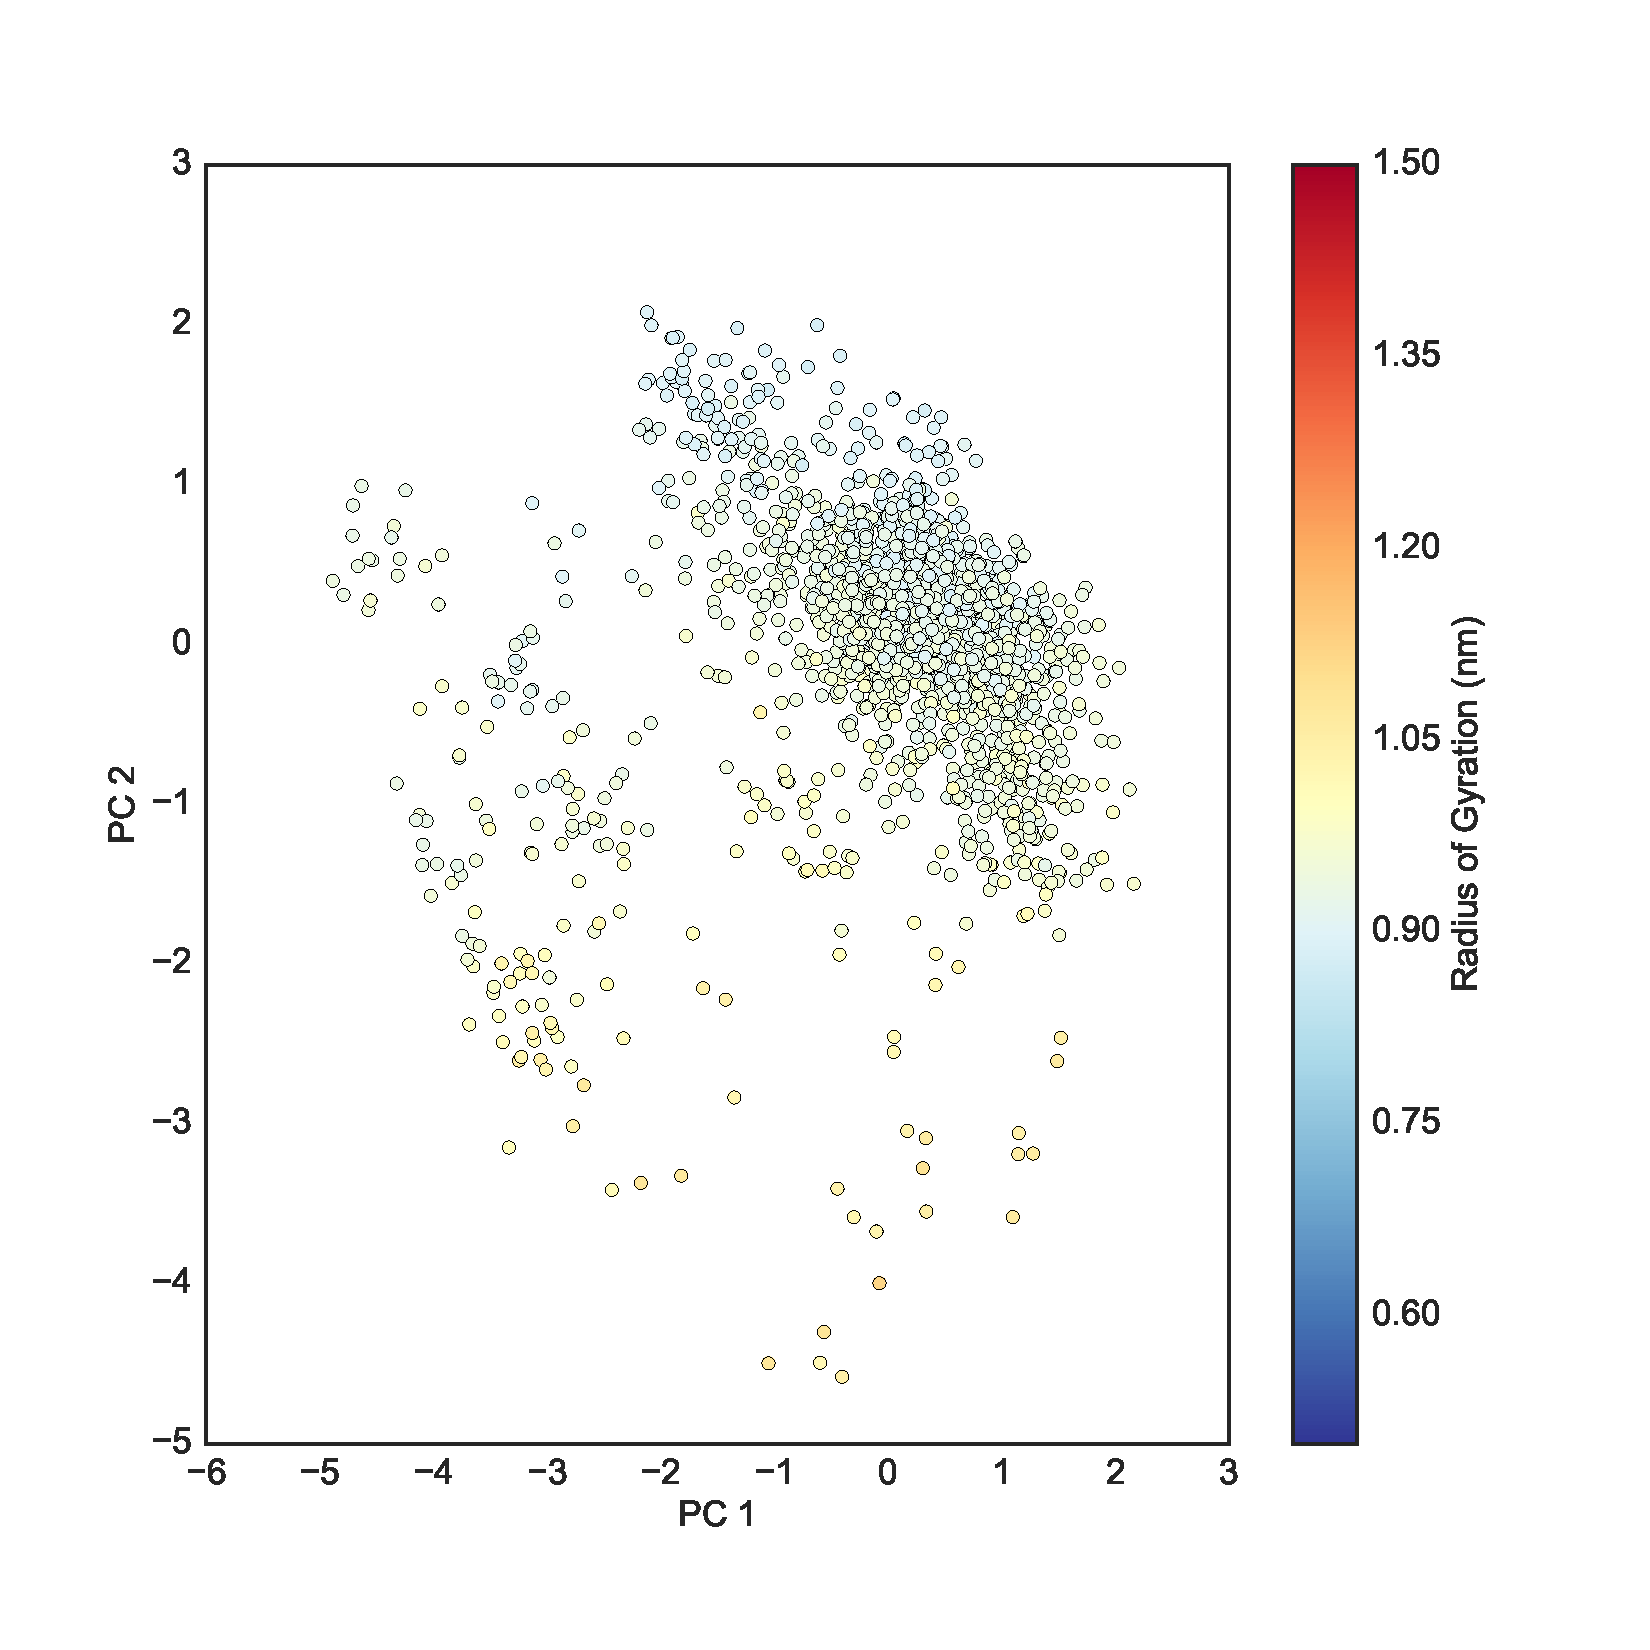
\includegraphics[width=0.49\textwidth]{2d_scatter_yd}} 
	\FigureCaption{Principal Component Analysis}{2 dimensional projections of the WT  \figref{fig:wtscatter} and YD trajectories \figref{fig:ydscatter}. Each point represents a 3D conformation projected along the first two principal axes. Conformations are colored according to a normalized \diffusion value where 1 is the lowest \diffusion (most extended) and 0 is the highest (most compact).}
	\clearpage
	\label{fig:pca}
\end{figure}

In order to visualize the transitions, we generate a porcupine plot depicting the direction of motion between conformations on two extremes of the second principal component projection \figref{fig:porcupine}.  We show that the transition between collapsed and extended is indeed driven by a separation of the N and C terminus in a correlated fashion. \todo{cosine content} With this analysis we are able to propose a physical mechanism to explain the concerted global dynamics and diffusion coefficient shift observed in NMR as the action of correlated motions brought about by a local change in electrostatic environment. 

%When choosing which component to use for the visualization we computed cosine content values of each projection. This has been shown to be an effective method for detecting the presence of diffusion in signals from trajectories which often dominate the first few eigenvectors. The only component with significantly high cosine content was the first principal component of the YD simulation and so we focus our attention on projections along the second component.

\begin{figure}
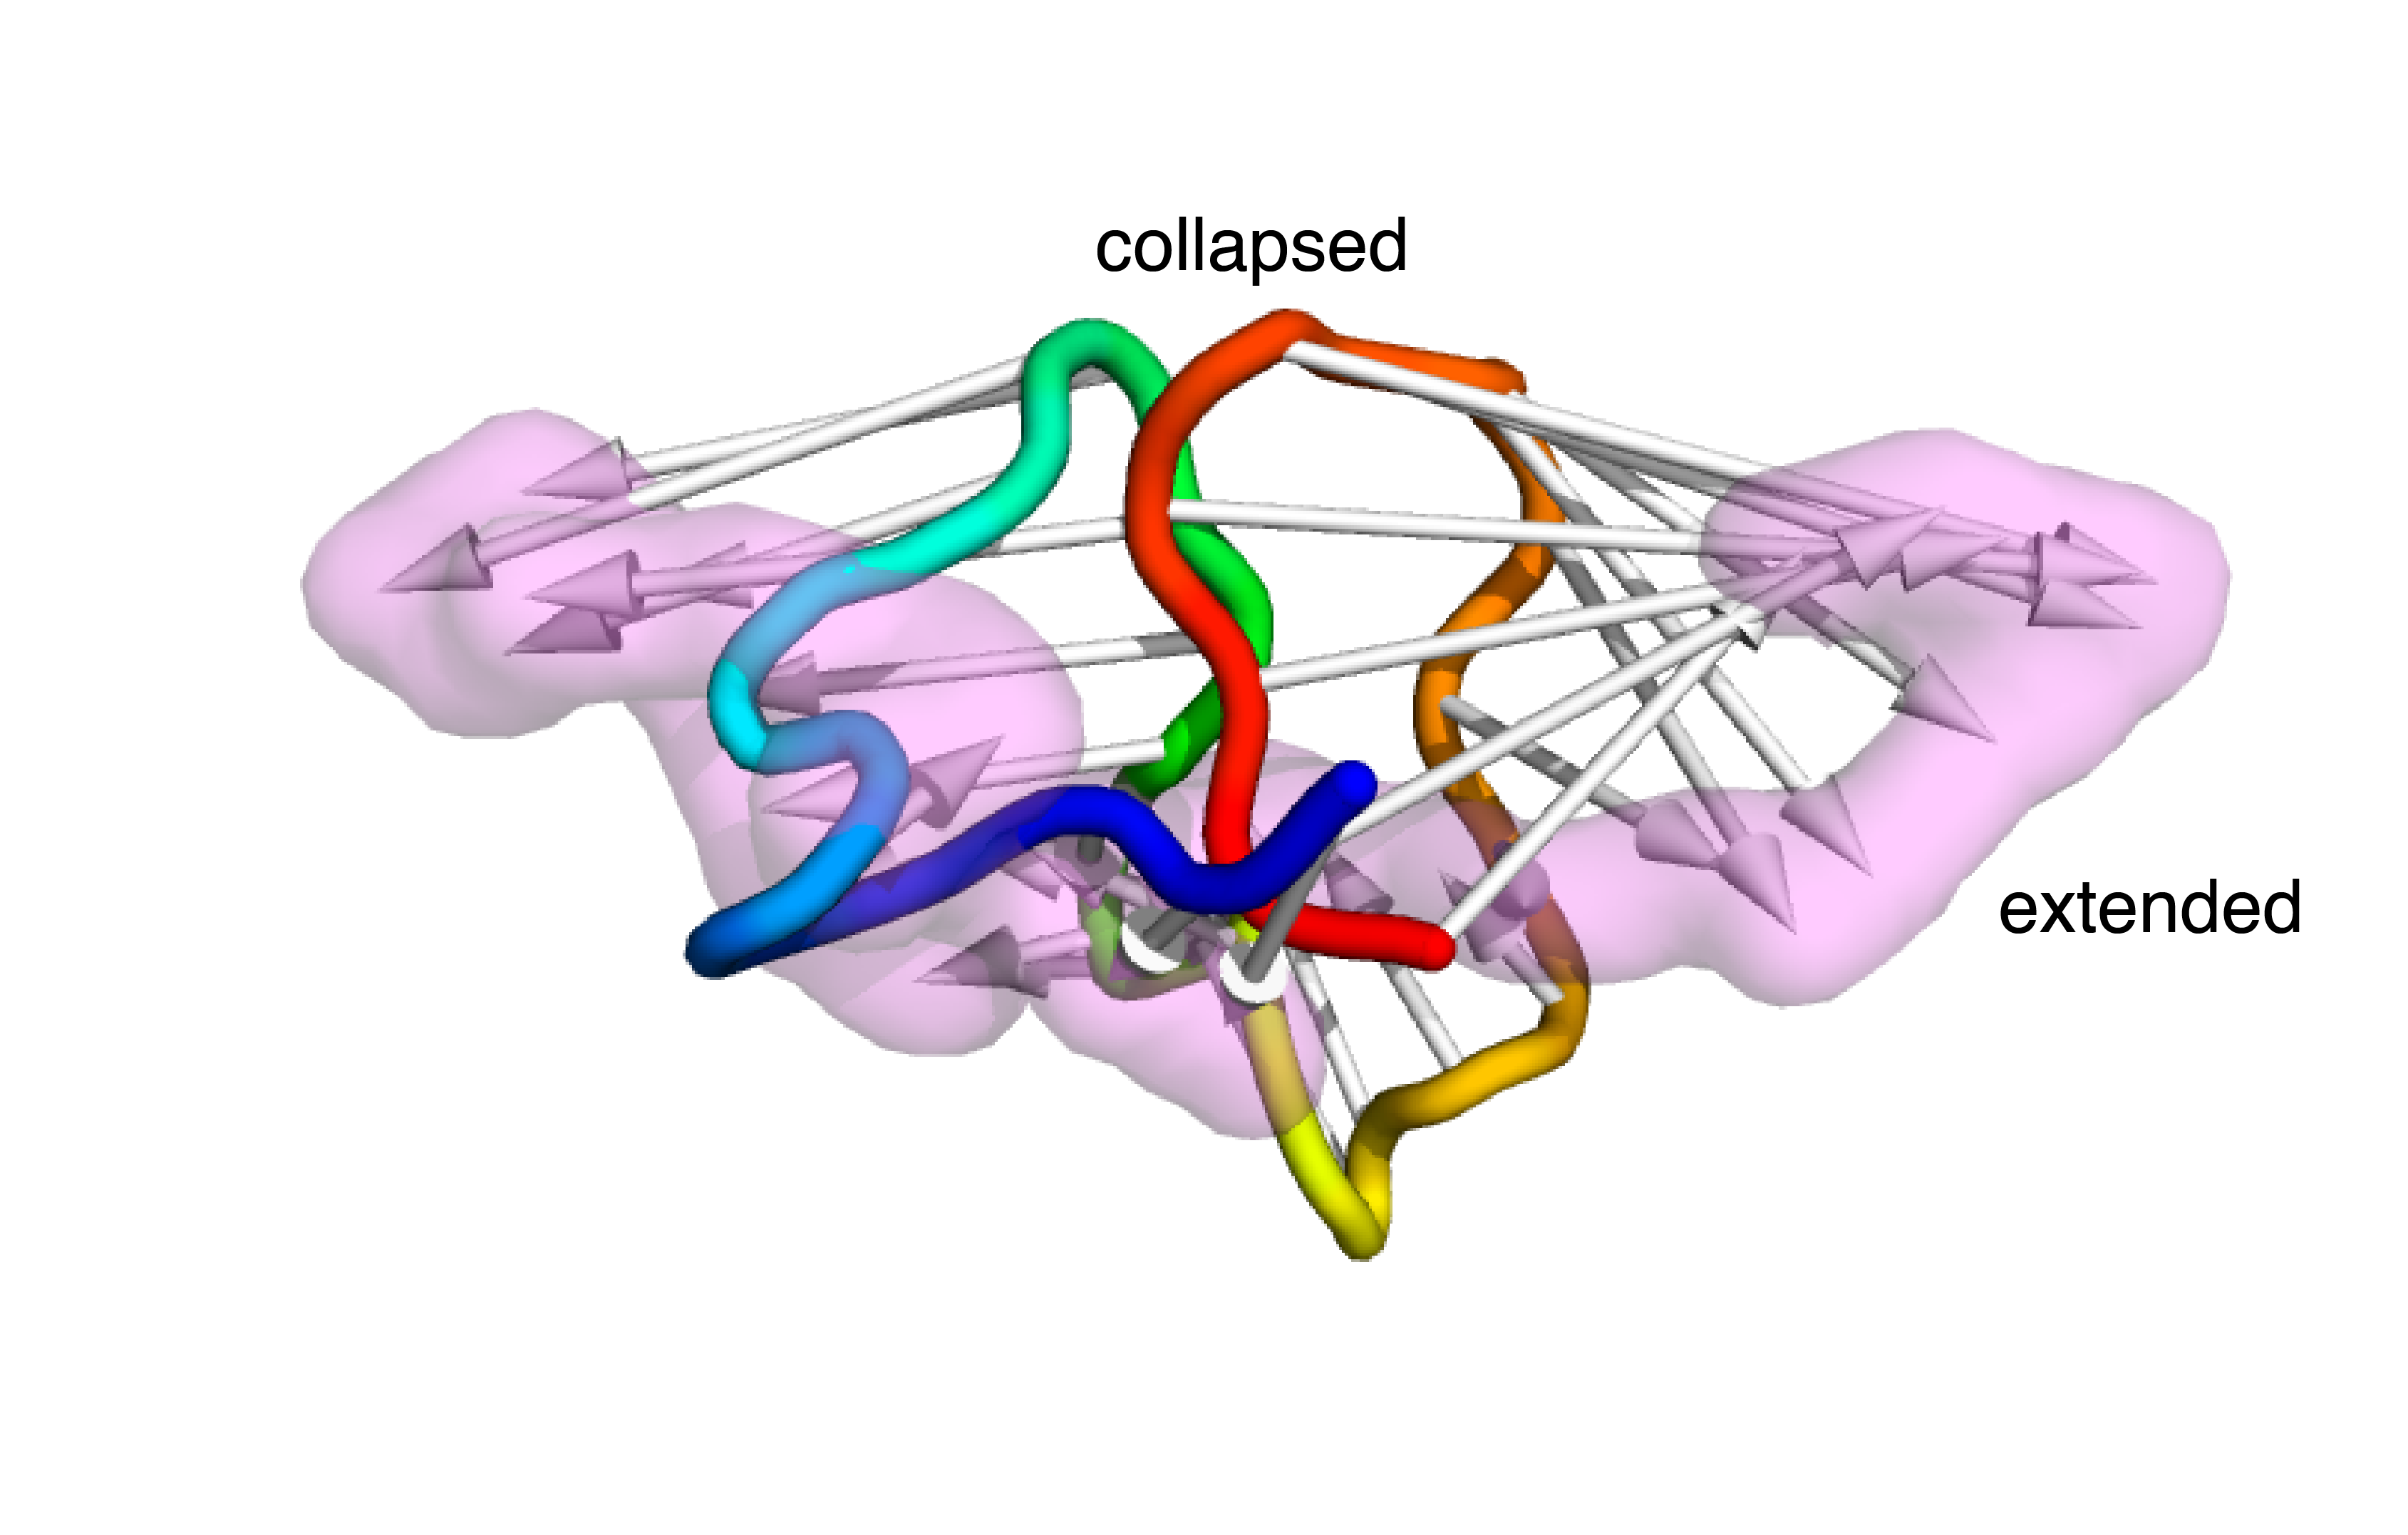
\includegraphics[height=0.4\textheight]{yd_porcupine}
\FigureCaption{Extreme projection along opening-closing axis.}{Arrows indicate direction of motion along opening/closing axis from YD PCA where the purple cloud represents the most extreme projection along the axis and illustrates the collective separation of N and C terminus.}
\label{fig:porcupine}
\end{figure}  


\subsection{Whole protein simulations and conserved properties of \gct}

Our analysis of \gct structural properties using NMR and corresponding MDS are based on the WT and Y11D \gct polypeptides in isolation. In order to determine whether the conformations and dynamics we observed for the isolated \gct are physically consistent when attached to the full-length \tub protein, we docked the minimum \diffusion \gct model \figref{fig:globular} onto the globular domain of an S.c. \tub homology model as an initial structure for a whole protein simulation. Due to the substantial increase in system size, simulation times were reduced to 200ns.  Despite the shorter simulation time, with the Y11D \gct polypeptide, the \gct in the whole protein simulation underwent exchange between extended and compact conformations \figref{fig:globular}, suggesting both states are still accessible in the presence of the globular domain. We found no contacts between residues in the globular domain with the 39 residues of the \gct throughout the 200 ns simulation (minimal distance between any pair of residues is > 0.7 nm) \todo{glob contact maps}. Structures for the full protein with the \gct at minimum radius of gyration (1.073 nm; model S11) and maximum radius of gyration (1.582 nm) are shown in Fig. 9A. This suggests that the \gct opening-closing mechanism can act independently of the rest of the protein.



\begin{figure}
	\thispagestyle{empty}
	\centering     %%% not \center
	\subfigure[Whole protein simulation conformers]{\label{fig:glob}\includegraphics[width=0.49\textwidth]{glob_overlay}}
	\subfigure[\gct Radius of Gyration]{\label{fig:globrg}\includegraphics[width=0.35\textwidth]{globrg}} 
	\FigureCaption{\tub whole protein simulation}{\figref{fig:glob} Alignment of whole protein simulation structures with mean, maximum, and minimum γ−CT radius of gyration. \figref{fig:globrg} radius of gyration of \gct from whole protein simulation. Shaded blue region denotes 1 standard deviation around t he mean radius of gyration value.}
	\clearpage
	\label{fig:globular}
\end{figure}


Finally, we obtain evolutionary evidence that the physical mechanism of the \gct described here is likely present in many other organisms, and that it is not akin to other tubulin tails.  We used the \texttt{MUSCLE} alignment tool \cite{edgar2004muscle} to generate multiple sequence alignments from sets of 71 $\beta$ and 85 $\gamma$- CTs primary sequences spanning various eukaryotic kingdoms from the UniProt database ~\cite{apweiler2004uniprot} \figref{fig:alignment}.  We see from the resulting alignments that both CTs are enriched in acidic residues (Asp, Glu). Whereas \gct across eukaryotes additionally contain clusters of hydrophobic or polar residues which are not found in $\alpha$- or $\beta$-CTs. Interestingly, the residues most broadened in Y11D NMR spectra, i.e. those most affected by the compact-to-extended transition (V15, D19, E20, A32, G34), are all found in positions conserved either on a sequence level or on a physical property level (polarity/charge) in the consensus \gct sequence. We therefore hypothesize that clusters of hydrophobic residues, including those that contribute to transitions between compact and extended conformations in the S.c. Y11 \gct, are a conserved feature of an otherwise diverse set of \gct s across many eukaryotic organisms. This feature appears to be absent in the well characterized $\beta$-CT "e-hook" domains which suggests that the \gct mechanism does not behave like its orthologues. \todo{talk about beta} Furthermore, given that the Y11 position is so pervasively conserved, it is likely that this mechanism of action is used by many other eukaryotes.

\begin{figure}
\centering
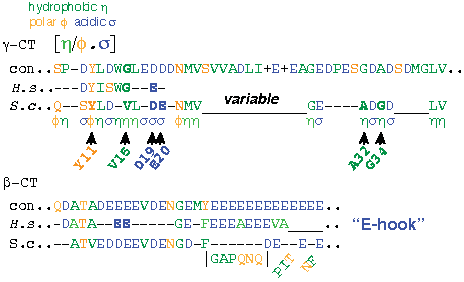
\includegraphics[width=0.7\textwidth]{consensus}
\FigureCaption{Multiple Sequence Alignment of \gct across eukaryotes}{Primary sequence consensus from a multiple protein-sequence alignment of \gct across various eukaryotes. Conserved physical properties are shown below primary sequence consensus (hydrophobic $\eta$, polar, $\phi$ acidic $\sigma$). An equivalent analysis is shown below for $\beta$-CTs, also known as E-hooks.}
\label{fig:alignment}
\end{figure}

\section{Discussion}

Through NMR measurements and MD computer simulations, we demonstrate the first example of an IDP acting as a disorder-to-disorder regulatory switch, and propose a physical mechanism to explain the regulation of an essential biological machine. 

Both NMR and MD are in strong agreement that the conformational sampling of the \gct lies entirely within the diordered ensemble, as no signal of secondary structure was detected by either method. Diffusion measurements show that the major conformational state of the \gct in the WT and in the YD is collapsed, with the YD having a slightly larger hydrodynamic radius on average. However, NMR and MD simulations both provide evidence that a single point mutation to a negatively charged residue Y>D produces concerted motions along the entire polypeptide that are not present in the WT \gct. Analysis of the collective motions detected in MDS by PCA correspond closely to transitions between collapsed and extended states which leads us to hypothesize that the changes in chemical environment detected in MDS and difference in hydrodynamic radius is a product of an correlated opening and closing motion brought about by the Y>D mutation. This coordinated opening is likely brought about by the effects of electrostatic repulsion as the Asp substituion introduces further negative charge in an already acidic region. It has been previously shown that charge has a strong influence on the conformational ensemble and diffusion rates in IDPs \cite{mao2010net}. Once the \gct enters the open state, several hydrophobic residues in the middle of the polypeptide(L464, A466, G468) become accessible for protein-protein interactions.

 Because both WT and YD appear to have the same collapsed native state and differ only when the YD undergoes transient excursion to an extended state, we can model such behaviour as a two well potential system \figref{fig:wellsb}. The equilibrium between extended and collapsed conformations is shifted by phosphorylation to render extensions more accessible in the YD.  Previously, such dynamics were only observed in the well characterized order-to disorder transitions, or the folding-on-binding paradigm ~\cite{tompa2012intrinsically}. Furthermore, this model stands in contrast to the existing view of disordered ensembles as uniform \figref{fig:wellsa} spaces of random coils ~\cite{mittag2007atomic}. And instead, we observe that the disordered landscape has some structure that IDPs can selectively explore  through PTMs to modulate functionality by giving rise to switch-like behaviour while still remaining disordered. Such behaviour likely presents advantages to the cell through its ability to provide high specificity and low affinity binding at a low entropic cost. This suggests for the first time that the disordered conformational landscape can be organized and can therefore play host to coordinated and functional transitions.

\begin{figure}
\centering     %%% not \center
\subfigure[Unstructured Landscape]{\label{fig:wellsa}\includegraphics[width=0.45\textwidth]{wells_a}}
\subfigure[Structured Landscape]{\label{fig:wellsb}\includegraphics[width=0.49\textwidth]{wells_b}}
\FigureCaption{IDP Conformational Landscapes}{\figref{fig:wellsa} shows an energy landscape as a function of radius of gyration (black to red) where a modification in the IDP would lead to a uniform conformational shift towards uniformly less compact structures centered around a single energy minimum. \figref{fig:wellsb} illustrates the behaviour observed in the \gct, where the energy landscape appears to have a two-well structure. This landscape, when combined with phosphorylation, renders a minor state accessible allowing for switch-like behaviour in the disordered ensemble.}
\label{fig:wells}
\end{figure}

From these findings we propose that phosphorylation at Y11 of the \gct acts as a regulatory switch to modulate protein-protein interactions. In order to better visualize this mechanism, we dock 3D structures obtained from full \tub simulations into cryo electron microscopy models of the $\gamma$-TuRC ~\cite{kollman2015ring} \figref{fig:turc} which previously lacked any information on the \gct due to its disordered nature. Based on this visualization we can propose a mechanism to explain the phenotype of hyper-stable microtubules in the Y11D mutants in vivo. The extensions that project outward from the complex brought about by the YD substitution, or phosphorylation, allow the $\gamma$-TuRC to selectively recruit effector proteins to the minus end of microtubules, making them available to the entire complex to subsequently act in regulating microtubule dynamics. The constitutive addition of negative charge in the YD mutant therefore shifts the equilibrium between the collapsed and extended states, leading to a misregulation of the recruitment of microtubule associated proteins and thus a defect in microtubule dynamics. The identity of the  protein(s) being recruited by the \gct remains an open question but there are several candidates known to affect microtubule stability and localize to the spindle poles \todo{which candidates} are currently being verified through various experimental screens. However, the characterization of \gct conformational sampling  is an essential fist step and a useful tool in identifying these potential interactors and understanding the complex mechanisms by which IDRs regulate large molecular machines.

\begin{figure}
\centering
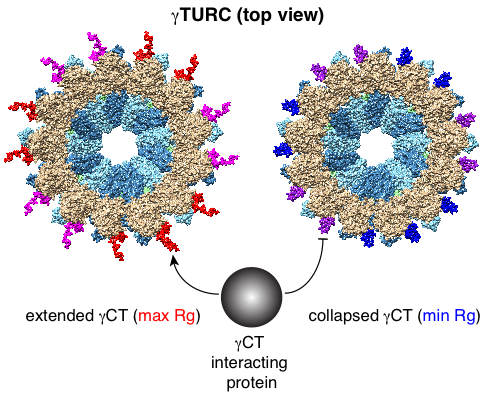
\includegraphics[height=0.5\textheight]{model}
\FigureCaption{$\gamma$-TuRC}{A working physical model for γ–CT selective interaction with accessory proteins through sampling between “extended” and “collapsed” conformations. Docking of simulated \tub models to $\gamma$−TuRC models shows a possible mechanism for regulating the binding of \gct interacting proteins to the ring complex. Extended (high radius of gyration) \gct complexes are accessible to interactions, while collapsed \gct  (low radius of gyration) inhibit interactions.
}
\label{fig:turc}
\end{figure}
